\documentclass{article}
\setcounter{secnumdepth}{0}

\usepackage{graphicx}
\usepackage{caption}
\usepackage{float}
\usepackage{pdflscape}
\usepackage{xcolor}
\usepackage[colorinlistoftodos]{todonotes}

\reversemarginpar
\captionsetup{justification=centering}

\title{Apprenticeship Portfolio}
\author{Oliver Matthew Bowker (220263618)}
\date{\today}
\begin{document}

  \maketitle
  \begin{center}
    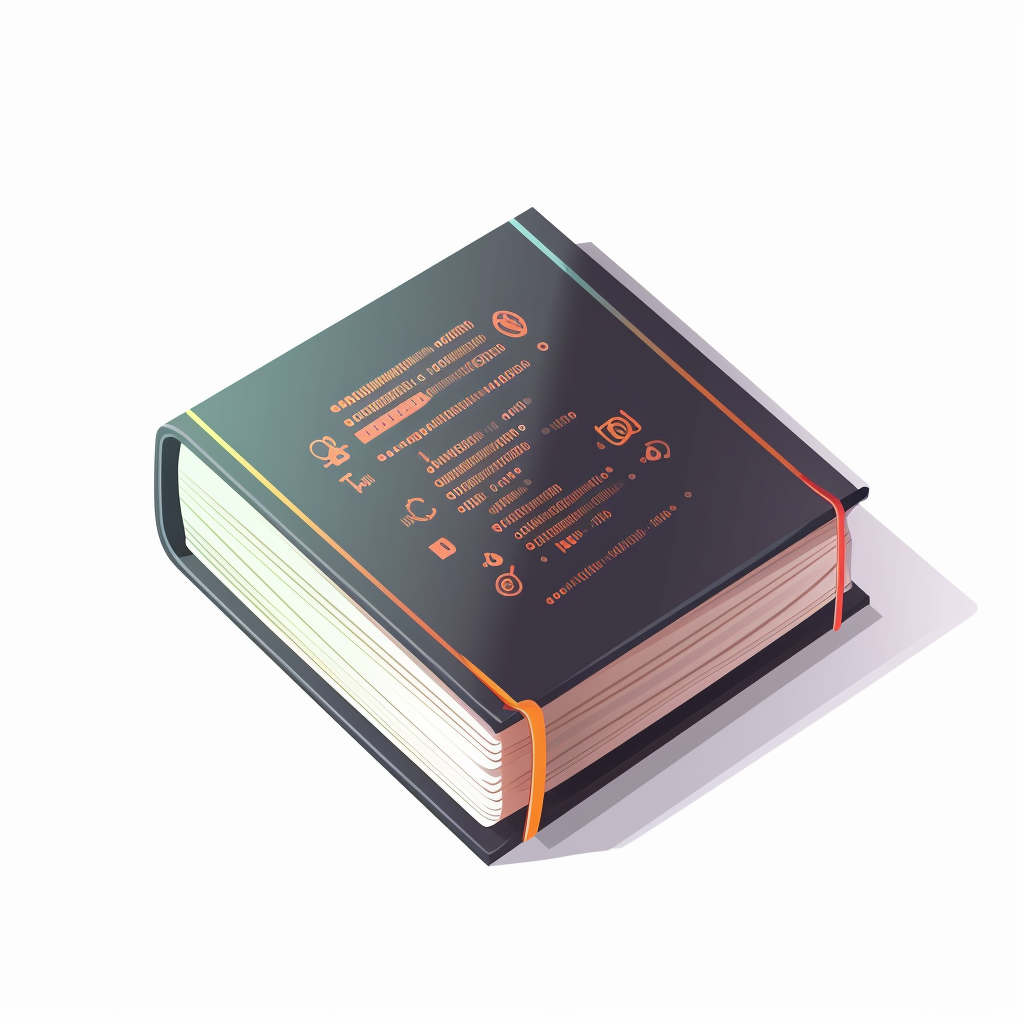
\includegraphics[width=5cm]{assets/cover.png}
  \end{center}
  \newpage

  \tableofcontents
  \newpage

  \listoffigures
  \newpage

  \listoftables
  \newpage

  \listoftodos
  \newpage

  \section{Projects}
  I will now briefly describe the two projects that will be discussed during this document/KSBs. More detail will be added to these projects throughout the
  multiple KSBs.
  
  \subsection{Off Product Inspector (OPI)}
  The Off Product Inspector (OPI) is a tool used by internal members of the BBC to view what media we offer to both internal and external partners. The tool 
  has two main functions:


  \begin{enumerate}
    \item To provide a search mechanism on all brand/series/episodes metadata that partners can access.
    \item To provide a tool that generates per partner specific links to catered or promotional data.
  \end{enumerate}

  The metadata we provide partners is written in JSON (JavaScript Object Notation) and can be hard to read, as a lot of the people are non-technical we provide
  a web based GUI for users to navigate and browse the data.

  \begin{figure}[H]
    \centering
    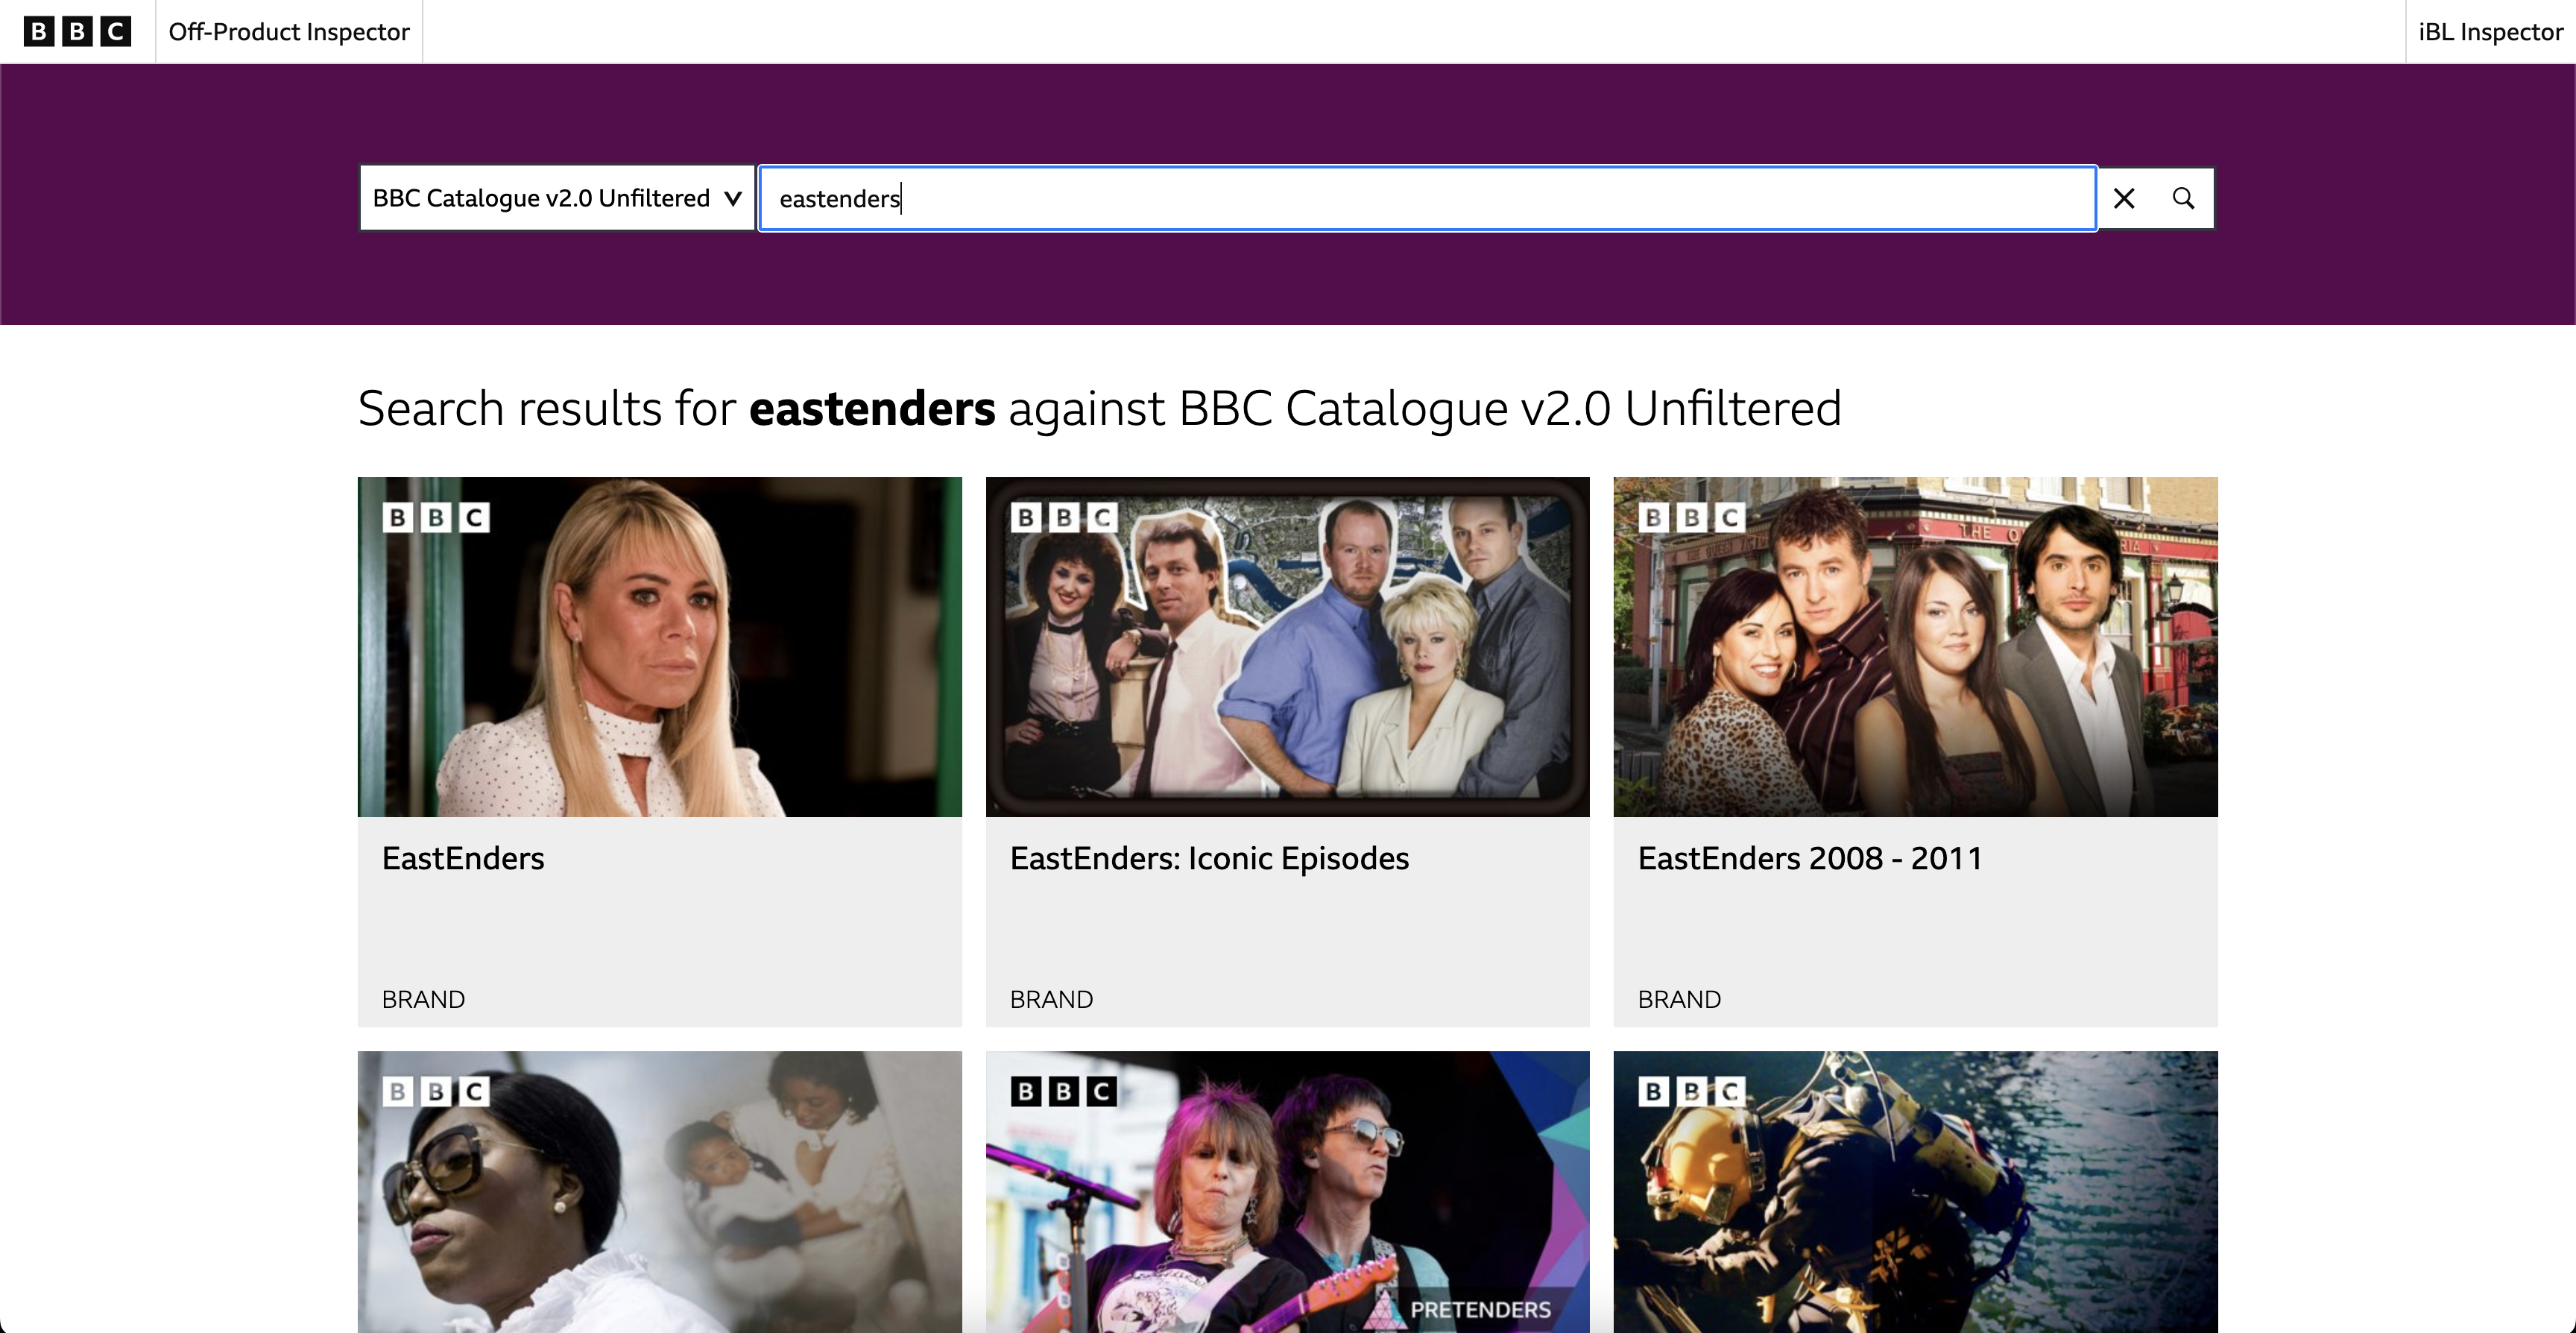
\includegraphics[width=6cm]{assets/OPI-search.png}
    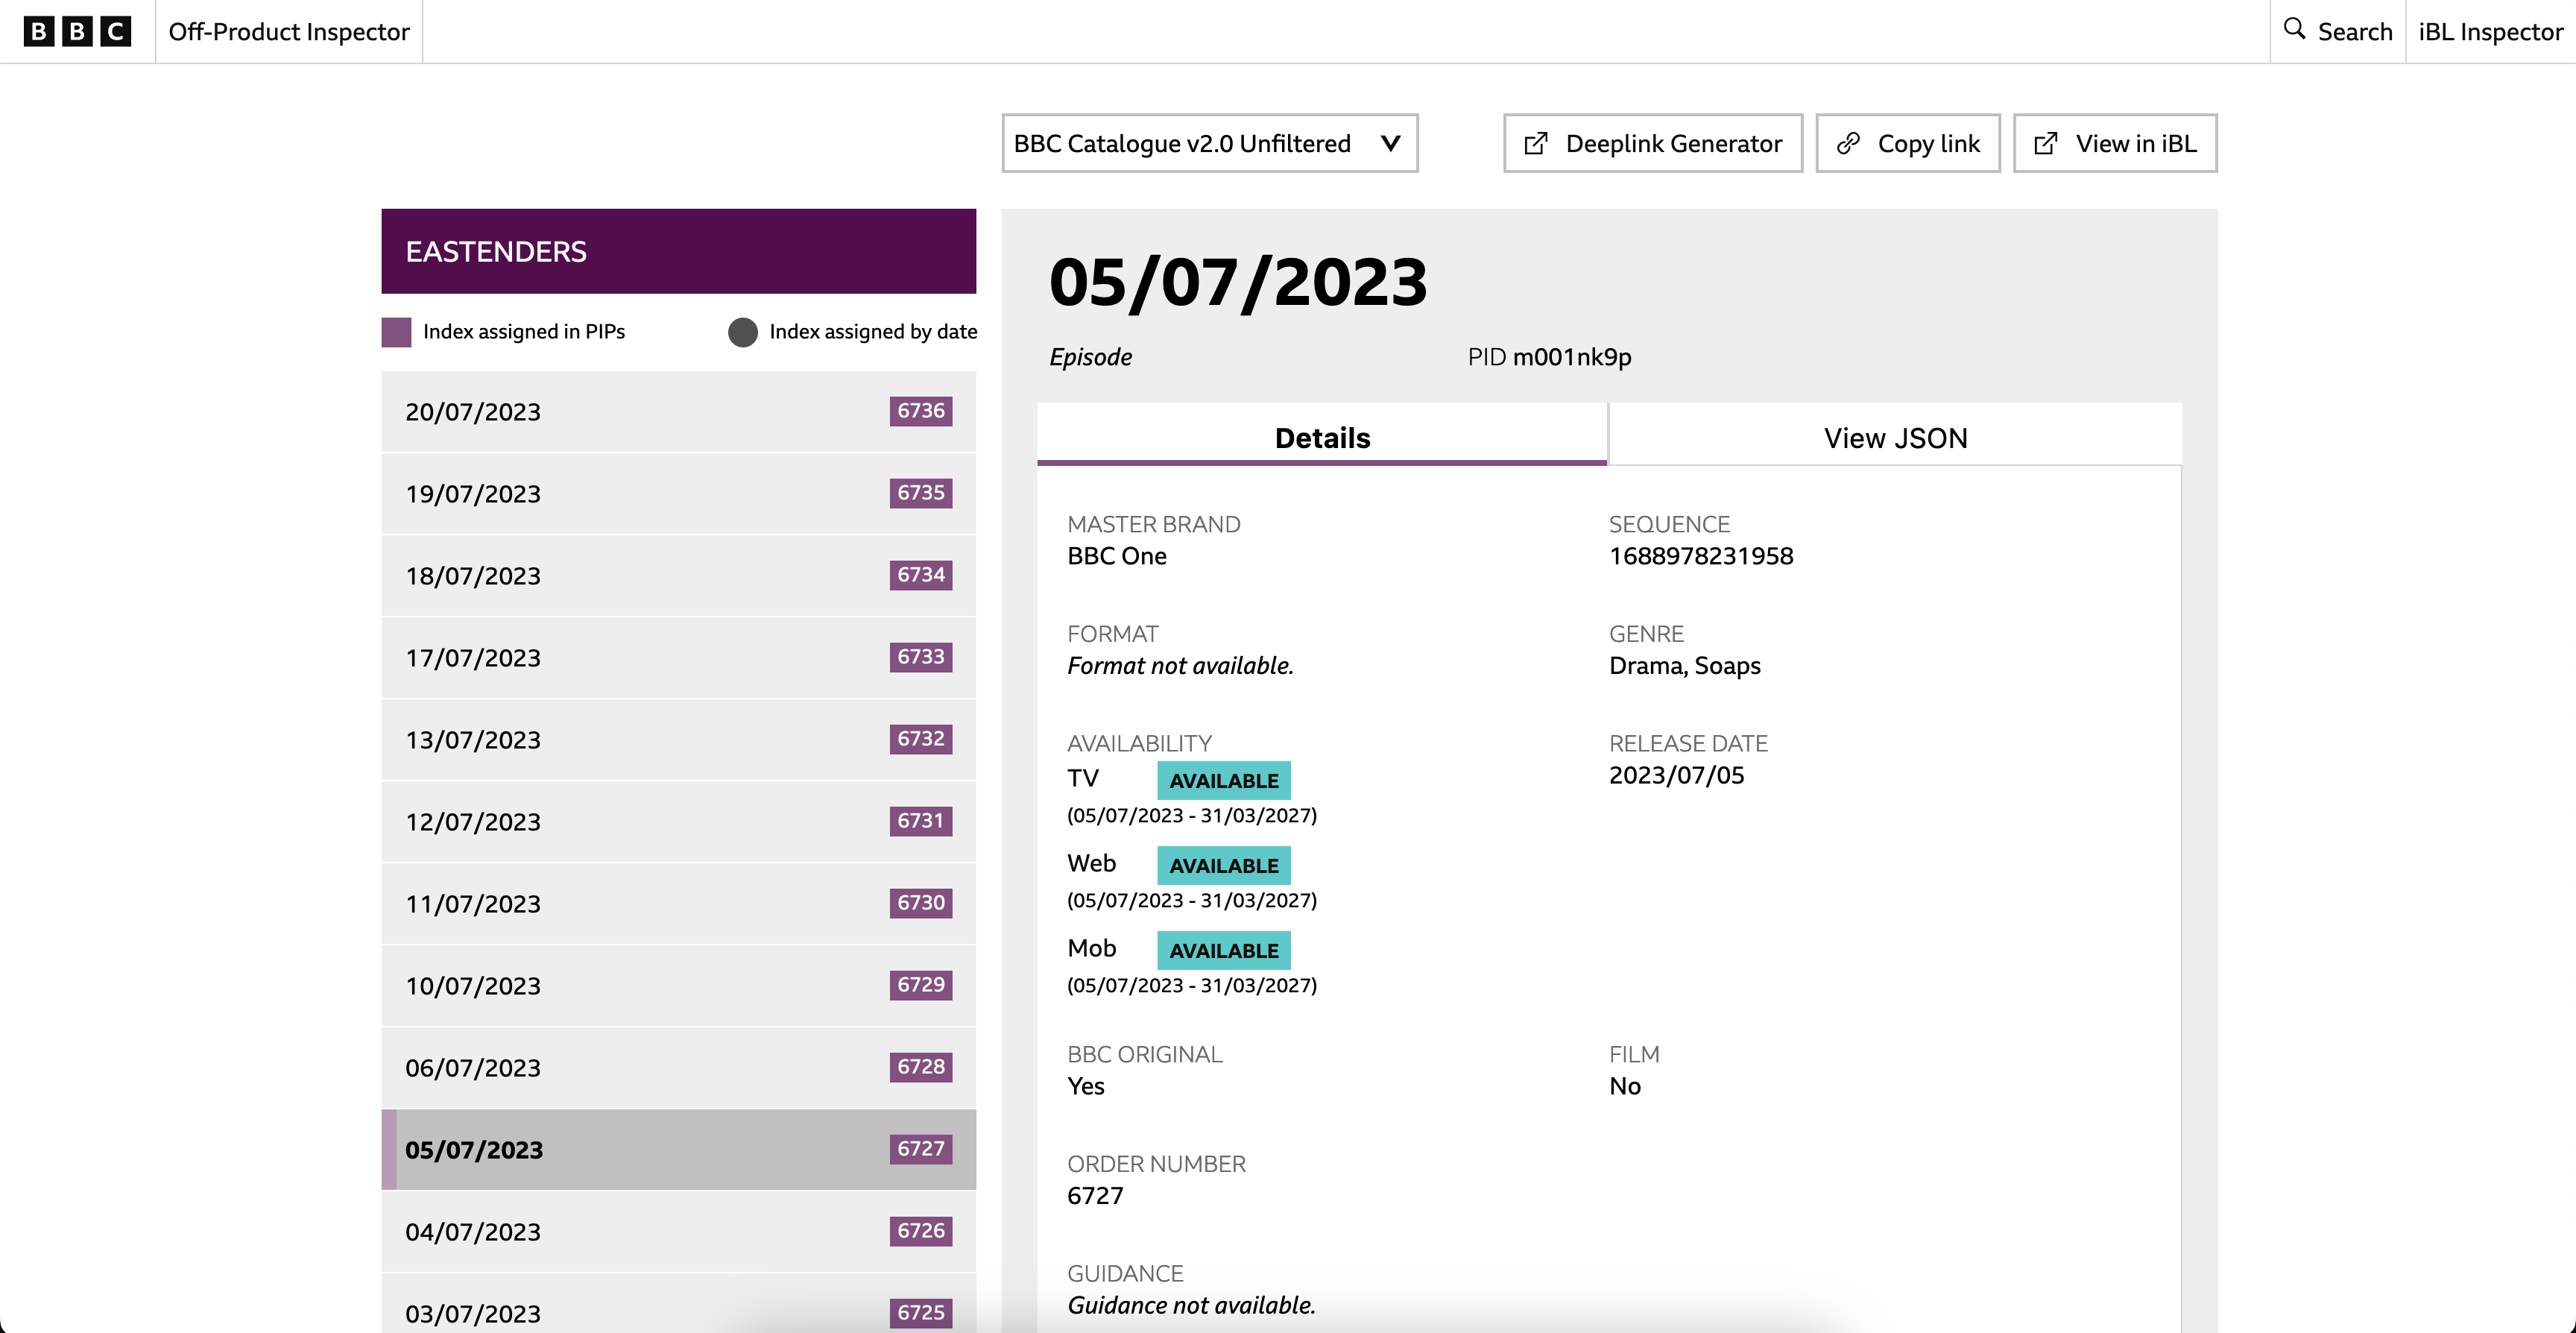
\includegraphics[width=6cm]{assets/OPI-detail.png}
    \caption{Screenshot of the search and episode/series/brand metadata viewer, (left-to-right)}
    \label{fig:opiMetadataOverview}
  \end{figure}
  
  The \textit{'Deeplink Generator'} is another part of the OPI that allows users to generate links to promotional/catered content. In the past links have been 
  malformed causing errors for partners, this tool aims to fix that by not having to manually write the links ourselves.

  \begin{figure}[H]
    \centering
    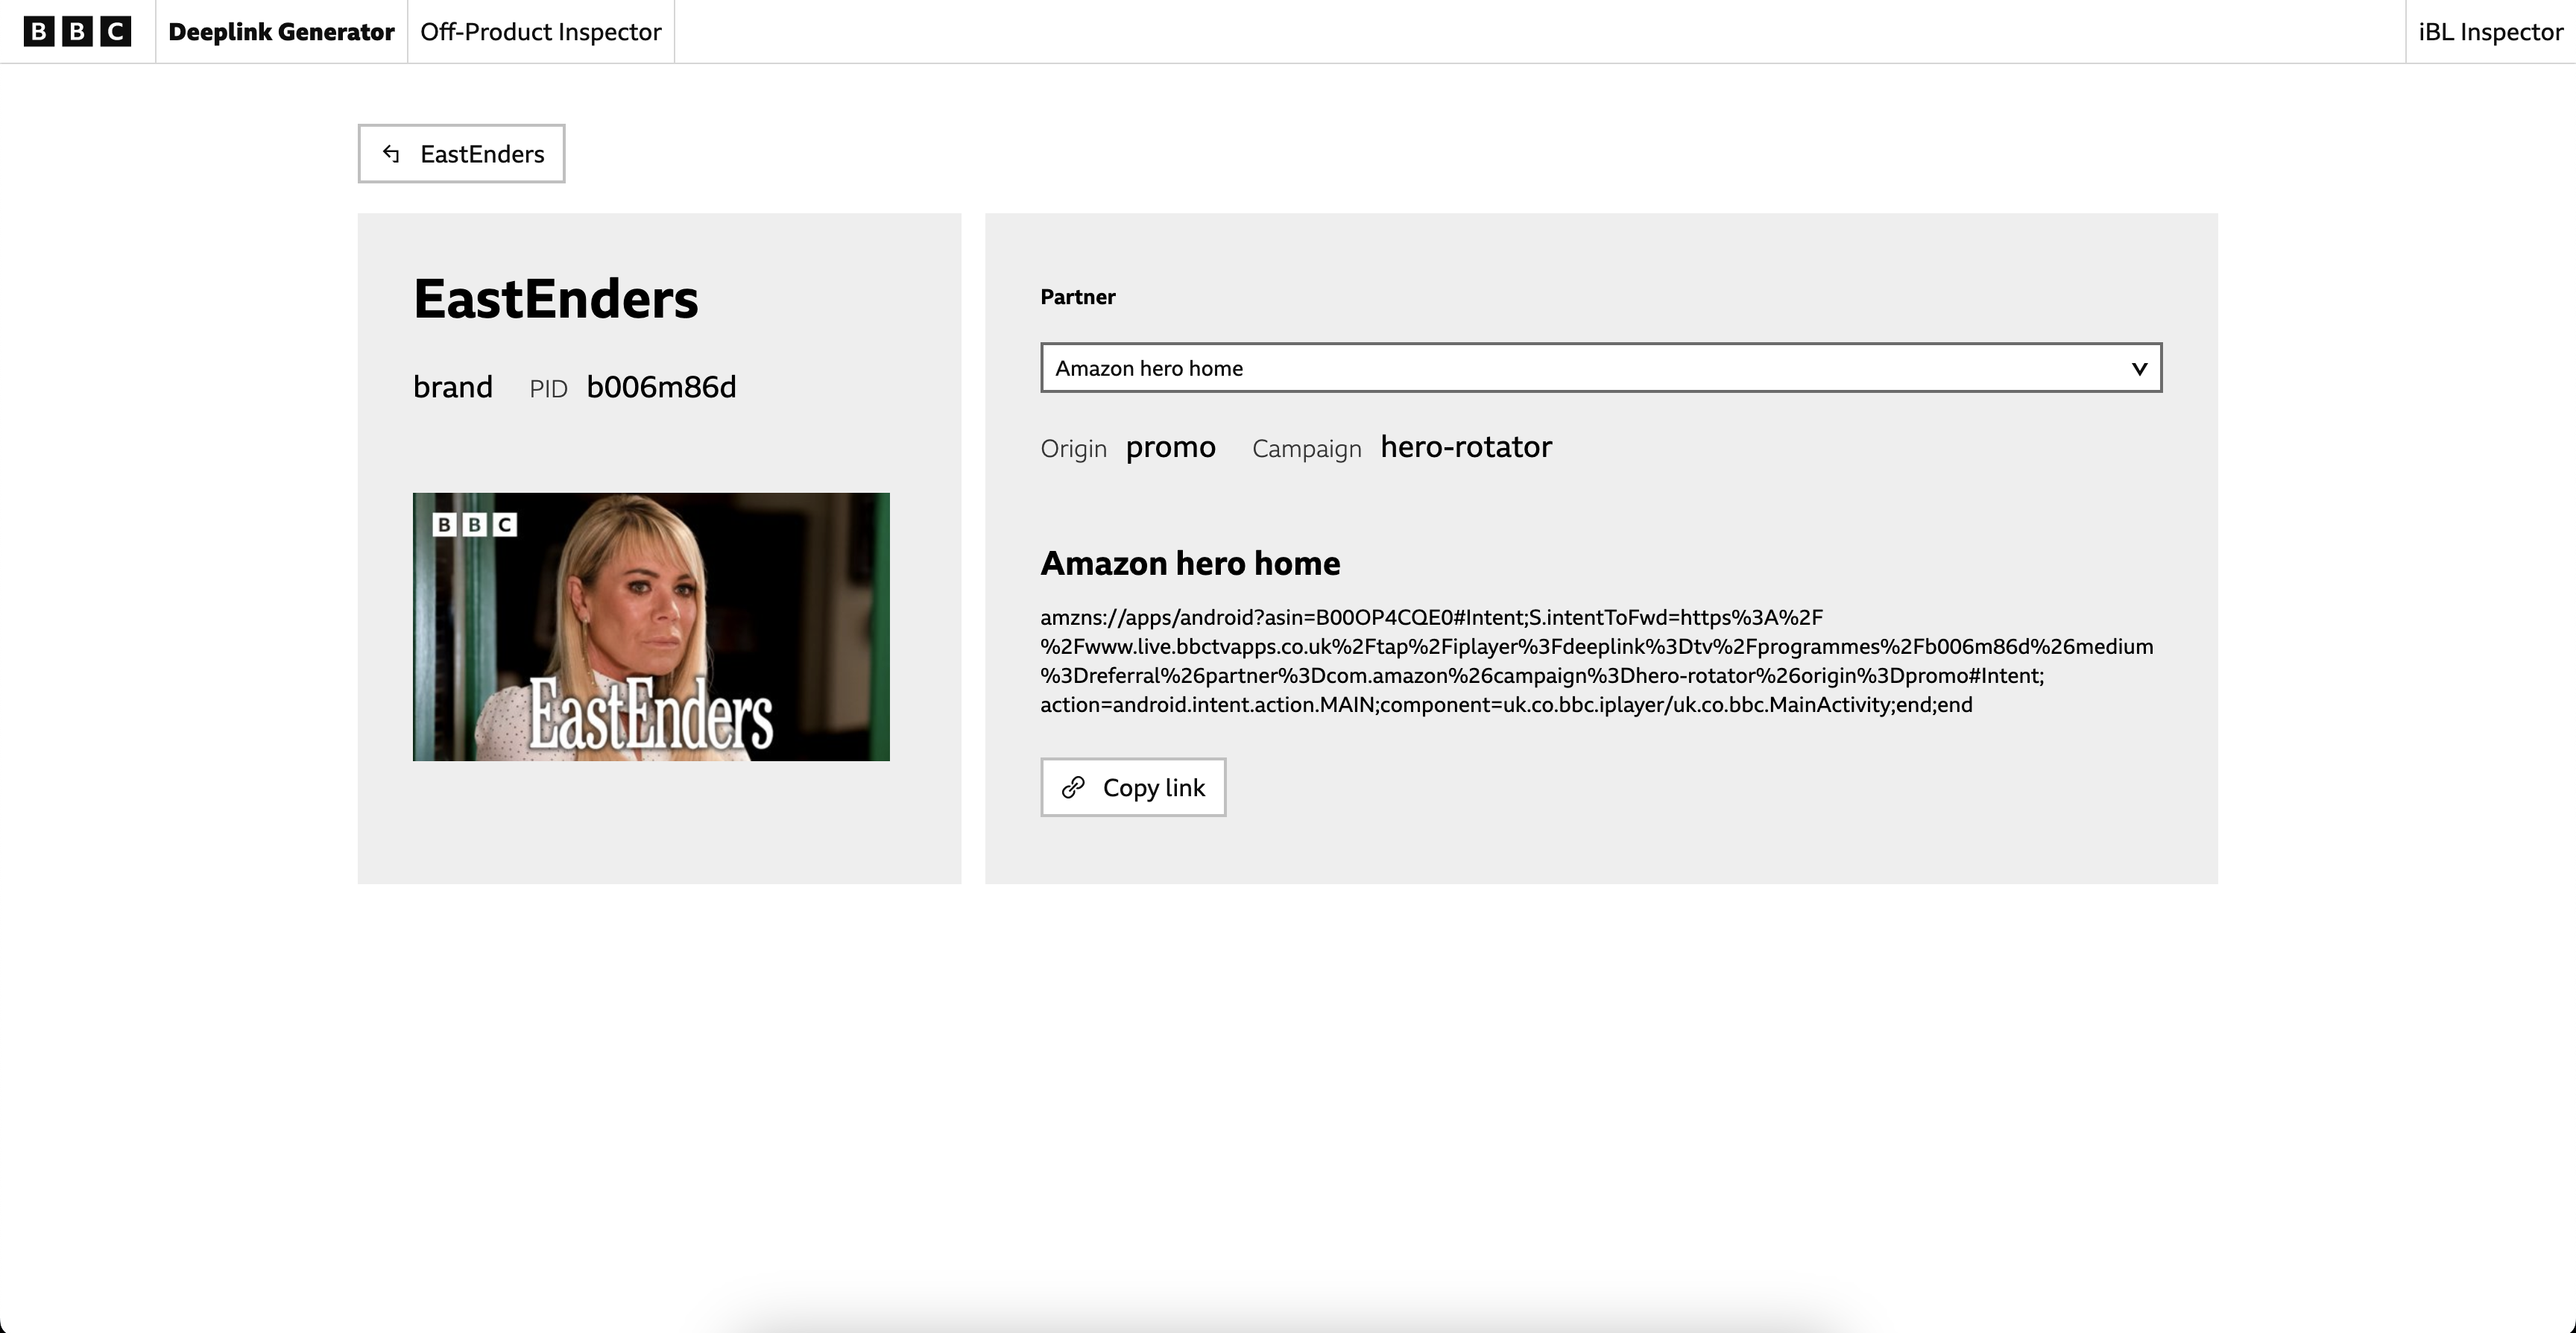
\includegraphics[width=6cm]{assets/OPI-deeplink.png}
    \caption{Screenshot of the Deeplink Generator tools}
    \label{fig:opiDeeplinkOVerview}
  \end{figure}

  \subsection{Schedules}
  The BBC plan to deprecate a service called \textit{'Nitro'} in order to save money on running the service and licenses attached to the service. As part of this
  certain data the service provided now has to supplied elsewhere. My team is responsible for supplying external partners with the schedule/EPG information.
  
  This data contains what is on linear television at what time, and also includes the aforementioned episode/series/brand metadata. In the real world this data
  is seen when you click 'guide' or corresponding button on the TV remote.

  \begin{figure}[H]
    \centering
    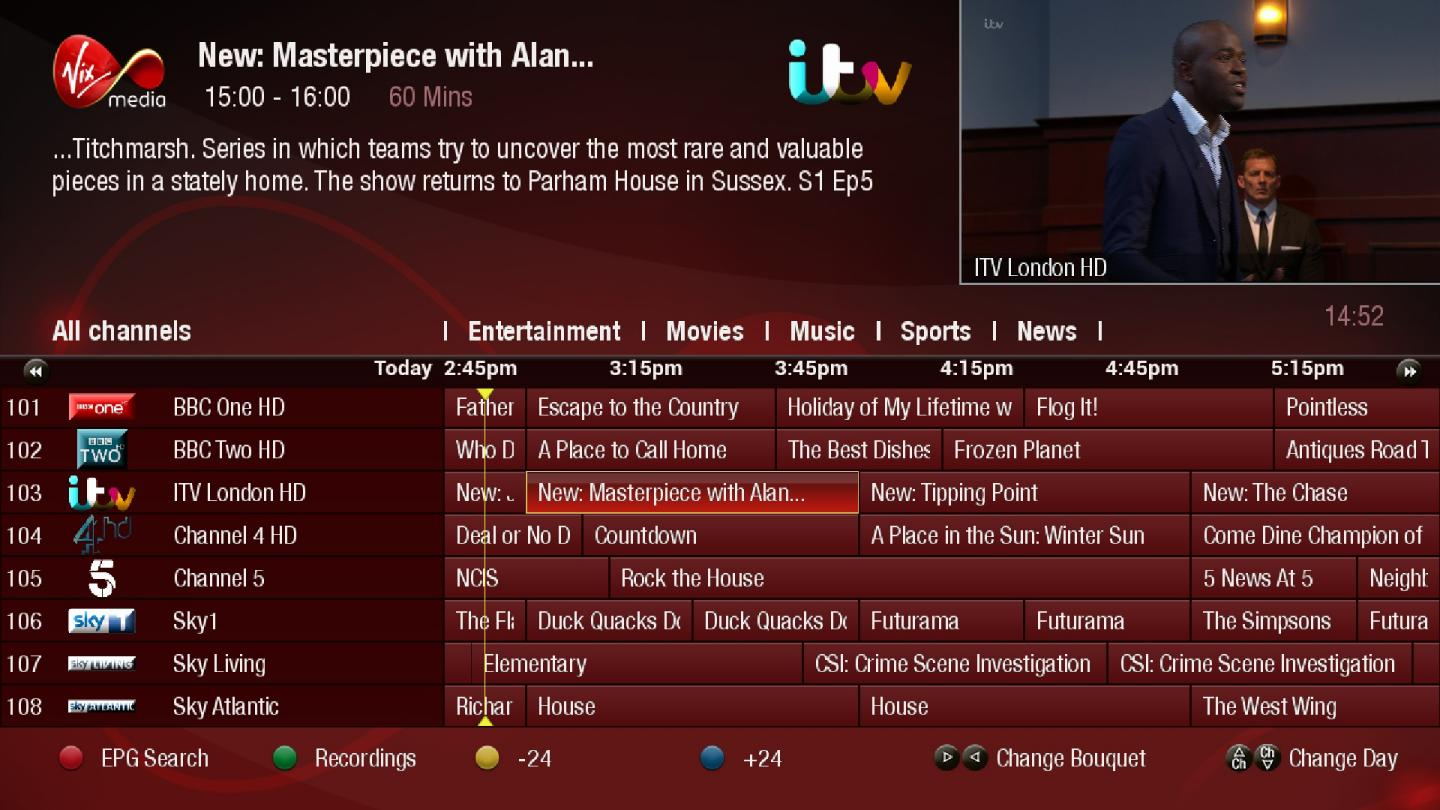
\includegraphics[width=8cm]{assets/epg.jpeg}
    \caption{Example of how EPG/schedules data can be used}
    \label{fig:epgExample}
  \end{figure}
  \newpage

  \section{Schedules}

  We have two pipelines, the \textbf{\textit{catalogue}} pipeline that is responsible for all the data that is currently accessible to partners on iPlayer
  and the new \textbf{\textit{schedules}} pipeline. We first have to ingest the schedule data from another source, which consists of over 1000 files and 
  then parse that data for what we want to share with partners. This parsed data is then stored in redis for future use. In the older catalogue pipeline 
  this process was done by an EC2 (server), however with this pipeline we wanted less to manage and decided to go with a lambda (serverless) approach. To speed 
  up ingestion of data we decided to experiment with multiple lambdas being invoked at the same time for concurrent processing of the files. 
  This is the part of the project I was tasked to document/create.
  
  \begin{figure}[H]
    \centering
    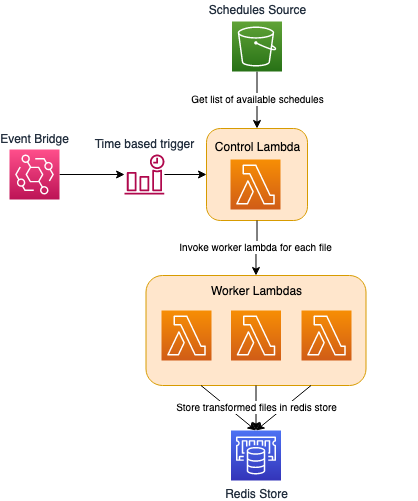
\includegraphics[width=6cm]{assets/ingester.drawio.png}
    \caption{Ingester AWS architecture.}
    \label{fig:ingesterArch}
  \end{figure}

  Figure 4 shows what the cloud infrastructure on AWS looks like. We get an event from event bridge, the available data is then retrieved from source and the
  parsing is then handed over to multiple concurrent lambdas. Finally this data is stored in redis for the next component in the pipeline to use. I have 
  illustrated this flow in the sequence diagram below.

  \begin{figure}[H]
    \centering
    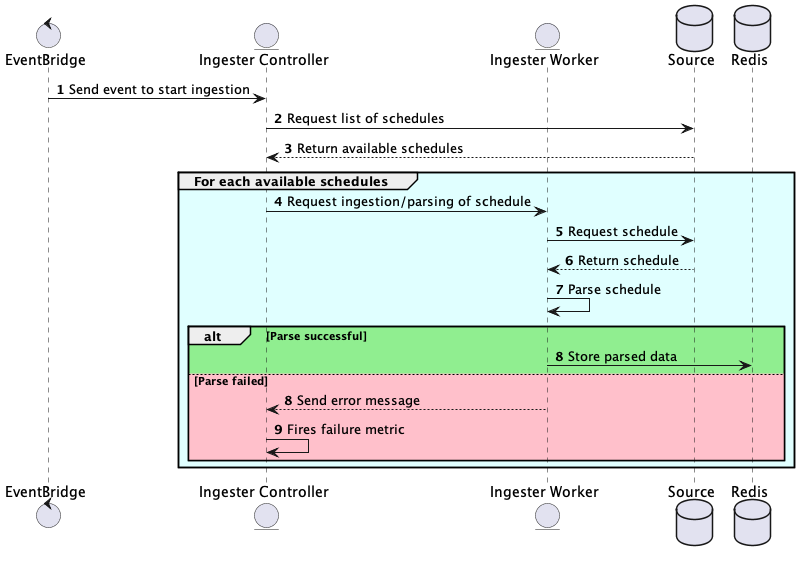
\includegraphics[width=8cm]{assets/diagrams/ingesterBasicFlow.png}
    \caption{Ingester basic execution sequence diagram.}
    \label{fig:ingesterFlow}
  \end{figure}

  For completeness I have also drawn a sequence diagram for the removal of old schedules from the redis store. This process is done just before the 
  parallelised lambdas are called to do their work. Removal is important here as if they were not removed it would have a knock on effect down the pipeline 
  as there would be unnecessary processing done for schedules that are no longer being used or accessible to partners.

  \begin{figure}[H]
    \centering
    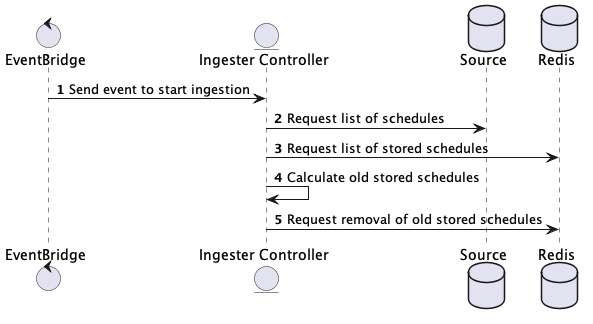
\includegraphics[width=8cm]{assets/diagrams/ingesterDataRemoval.png}
    \caption{Ingester old data removal sequence diagram.}
    \label{fig:ingesterScheduleRemoval}
  \end{figure}

  In the pipeline there is a second component called the \textit{Schedule Generator} that is responsible for outputting the data in a format partners will
  receive. For this component we did not have the worker lambda, and instead had a single lambda do all the processing. The two graphs belows show the 
  difference in lambda runtime between the two components.

  \begin{figure}[H]
    \centering
    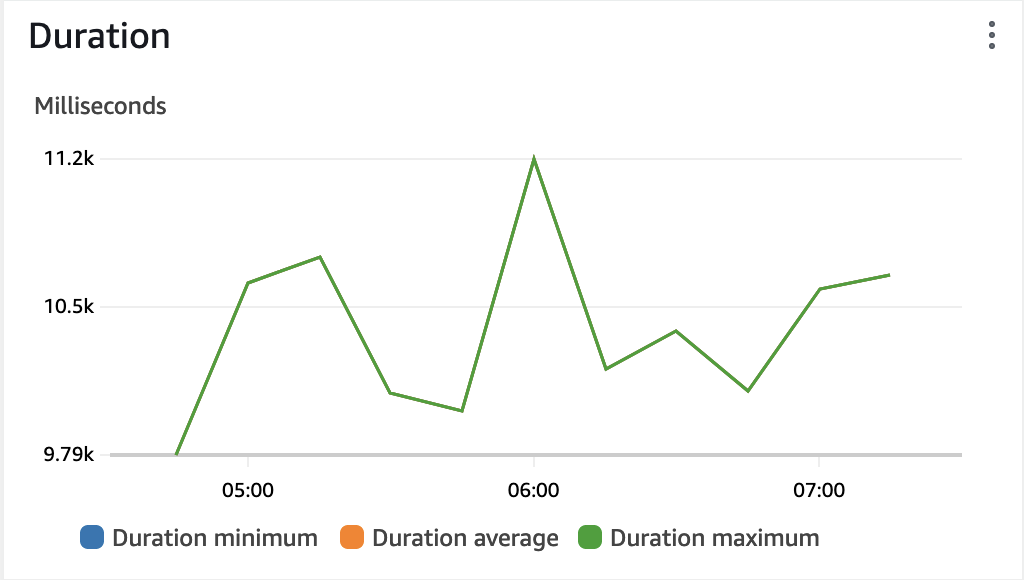
\includegraphics[width=6cm]{assets/ingesterDuration.png}
    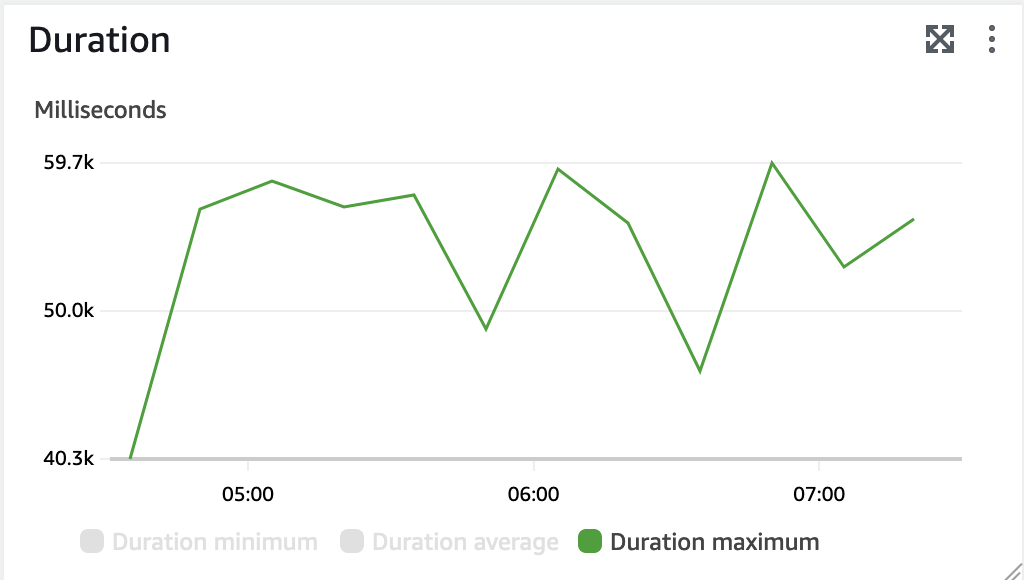
\includegraphics[width=6cm]{assets/generatorDuration.png}
    \caption{Screenshot of AWS lambda duration for schedule Ingester (left) and Generator (right).}
    \label{fig:lambdaDurationDifference}
  \end{figure}

  As can be seen, using parallelised lambdas is 4x quicker on average than using a single lambda. This is important as the quicker this pipeline can run
  the 'fresher' the data is for partners. After seeing these results there is now some talks about also changing the Schedule Generator to use the same 
  pattern.

  \vspace{0.2cm}

  This was also the first project where we upgraded to using the new version of the AWS SDK. This was something we hadn't looked into however was something
  that would be beneficial when we had to upgrade to node 18. AWS would no longer package version 2 of their SDK by default in lambdas. This would result in
  \todo[noline, size=\small]{L3, T2}
  an extra ~70MB of unpacked data being added to the final build which would slow down our build time and cost us a little bit more money, albeit fractions of
  a penny. I lead the investigation into using the new SDK and if it was feasible. This upgrade then also lead to the upgrade of our credentials provider
  which had security vulnerabilities that needed fixing.

  \begin{figure}[H]
    \centering
    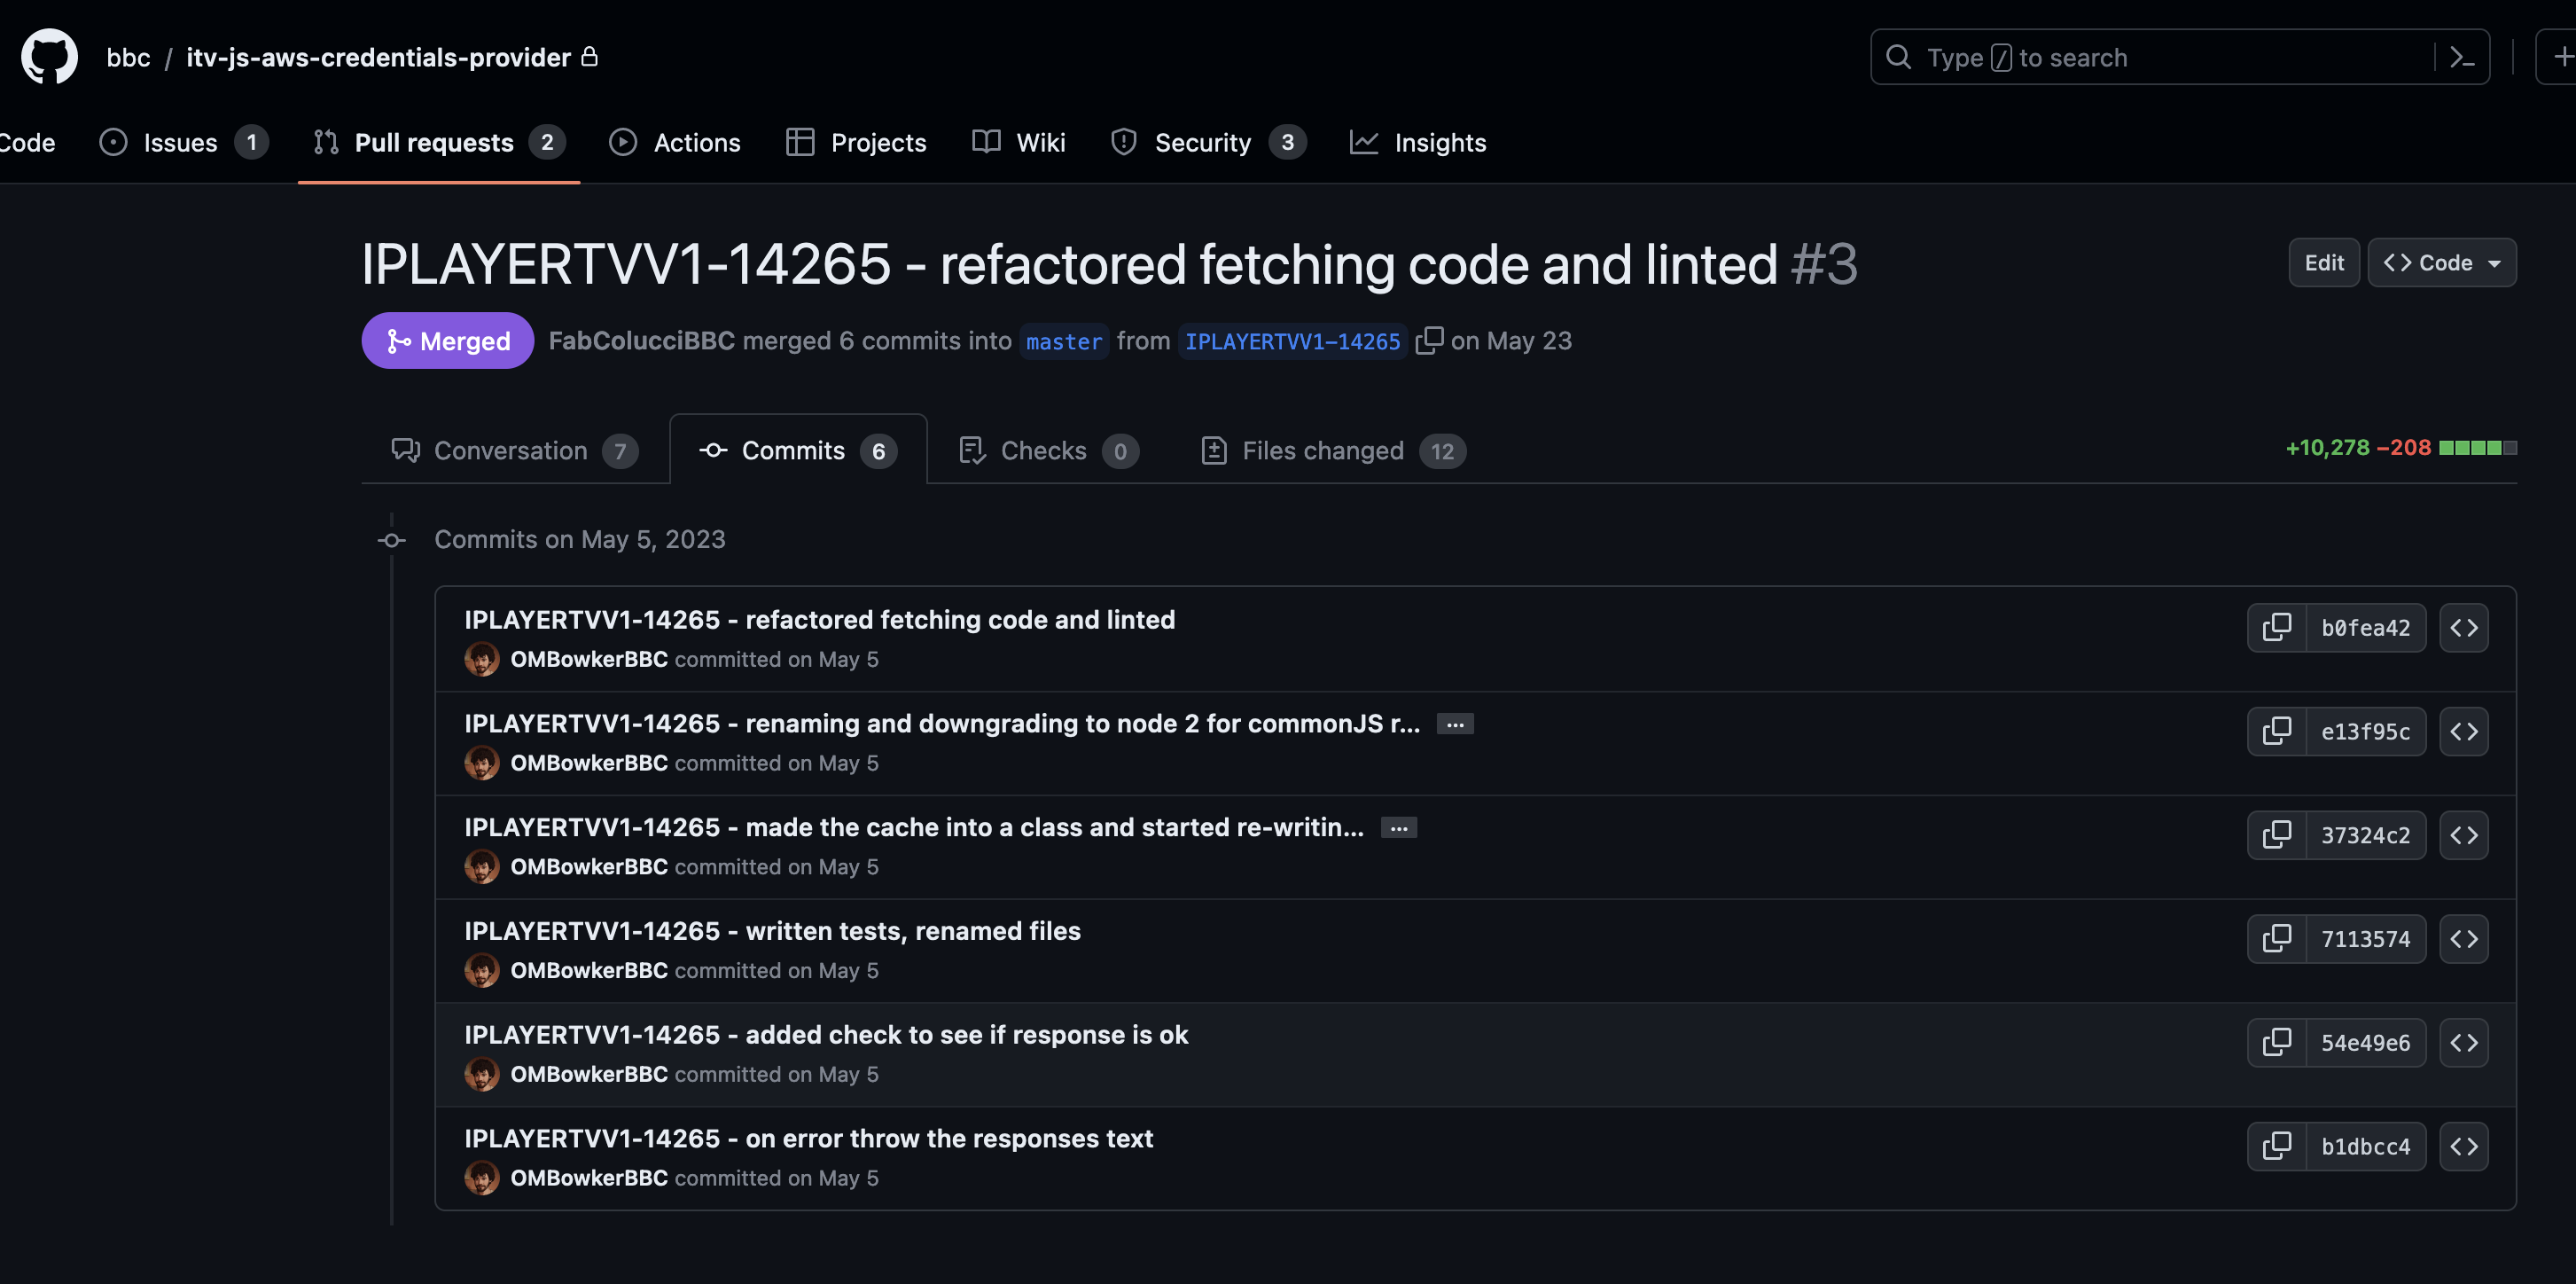
\includegraphics[width=6cm]{assets/credentialsRefactorCommits.png}
    \caption{Screenshot commits for credentials refactor.}
    \label{fig:credentialsRefactor}
  \end{figure}

  \subsection{The reason for schedules}
  Schedules is part of a much larger BBC wide objective to deprecate an external service called Nitro. The deadline for this is October with 
  schedules at the being retrieved from the service that wants to be deprecated. This switch to an internal system will give the BBC more 
  control/oversight of the data, directly contribute to one of our OKRs, (Simplifying Platform), these can be seen in \textbf{ContextSetting.pptx}, 
  and will also save us money in the long run.

  \todo[noline, size=\small]{B6}

  Previously partners were getting there data from this data source, but can now get the same, or even more rich data, from us directly. This can 
  help us with other OKR, like \textit{'Improve our data capabilities'} as it is much easier to track and analyse data that is requested from our 
  own service.

  \subsection{Burn-up charts and planning}
  \todo[noline, size=\small]{B2, P1}
  As schedules was a time sensitive project, it was important that we stayed on track with our work. To help with this our delivery manager 
  used some tools/techniques to visualise and clarify where we were at in development, but also what was to come next. Below is our roadmap
  for the schedules work.

  \begin{figure}[H]
    \centering
    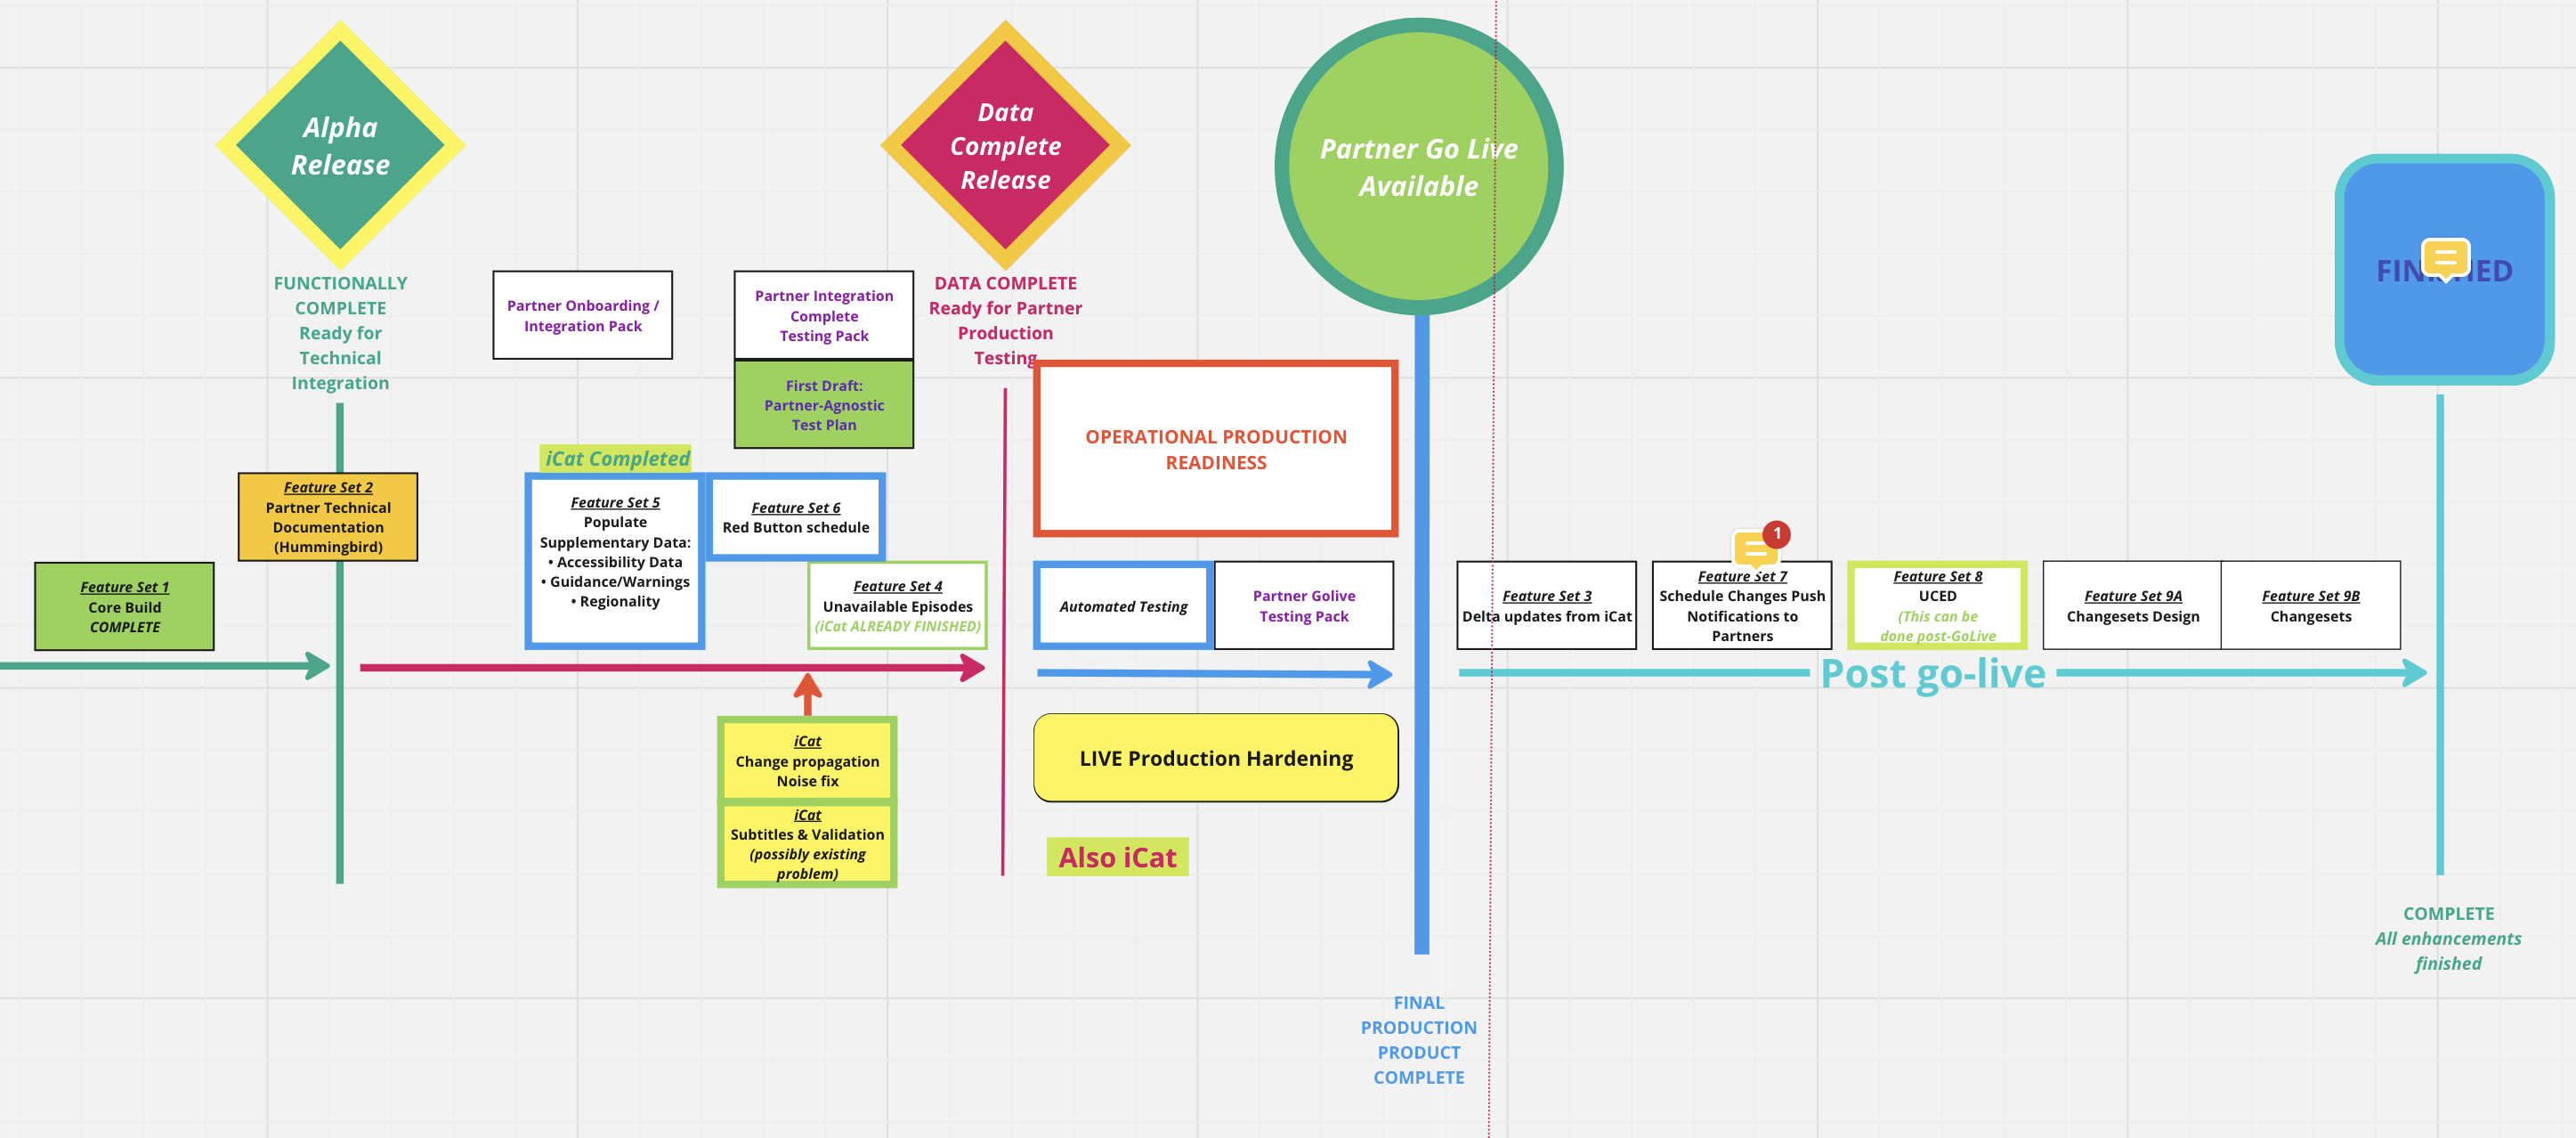
\includegraphics[width=10cm]{assets/schedulesRoadmap.png}
    \caption{Roadmap for schedules.}
    \label{fig:schedulesRoadmap}
  \end{figure}

  We have 4 stages \textit{'Alpha'}, \textit{'Data Complete Release'}, \textit{'Partner Go Live Available'} and \textit{'Finished'}.
  As of writing this we have completed the third stage, meaning that partners are now integrating and using the service. During the 
  creation of this there were many discussion of what needed to be done before each stage was complete.

  An example of this was the creation of automated tests, which would help validate our pipeline was parsing and sending the data to partners correctly.
  This was pushed back to just before partners could go live, but partners would already have access to the information for testing 
  on their systems. This was done as integration can take a long time, with a deadline of October it was vital that partners could start
  working with the data as fast as possible, however we felt that before we could go live we needed the assurance the automated 
  tests would provide us.

  Another discussion was around \textit{'deltas'}, which provide real time updates to the data, instead of a periodic update (every
  15 minutes). After some investigation and discussions it was decided that this was not needed to go live and could be added after, this due again 
  to time constraints but also the relevance of the changes would not be that impactful that the partner needed immediate updates.

  \vspace{0.2cm}

  In addition to roadmapping our delivery manager also used burn-up charts throughout the development of the project. Atlassian describes a
  burn-up chart as:

  \begin{quote}
    \textit{'The Burnup Chart provides a visual representation of a sprint's completed work compared with its total scope. It offers insights 
    on your project's progress, as well as offers warnings to help you maintain your project's health; you can instantly identify problems such 
    as scope creep or a deviation from the planned project path.'} [TODO1]
  \end{quote}

  The burn-up charts can be seen in the following images.
  
  \begin{figure}[H]
    \centering
    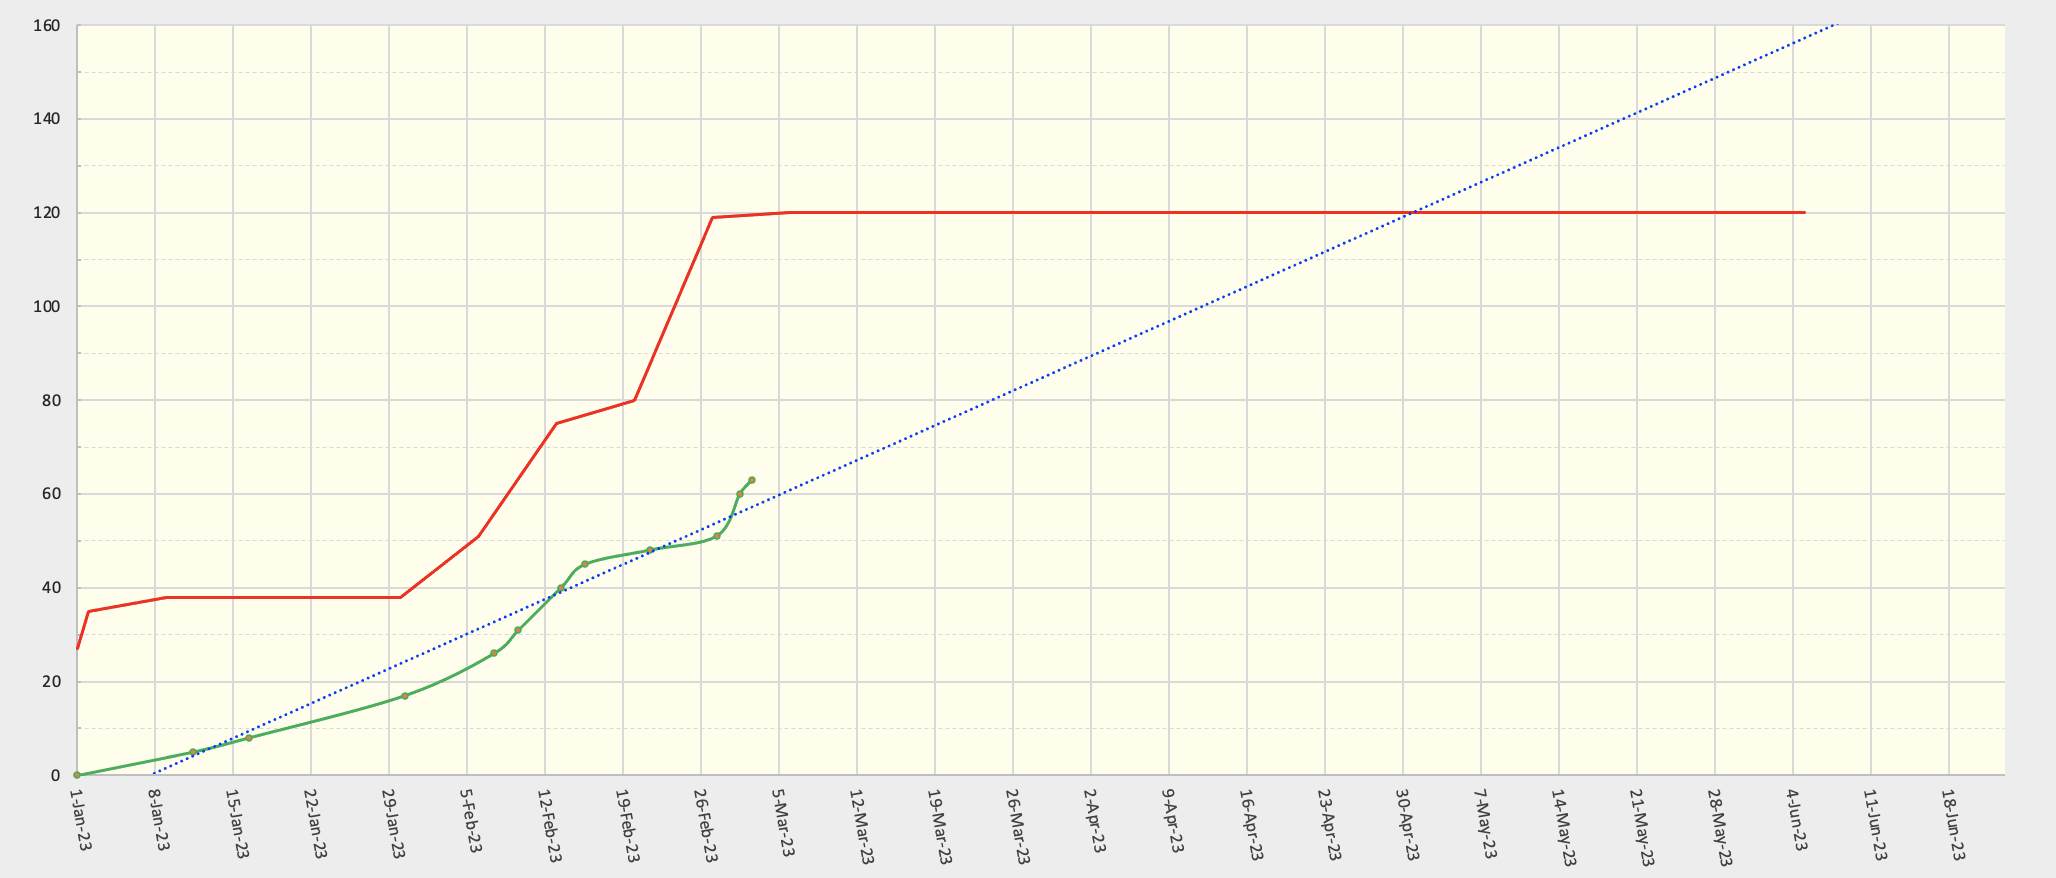
\includegraphics[width=6cm]{assets/burnup/2023-03-03.png}
    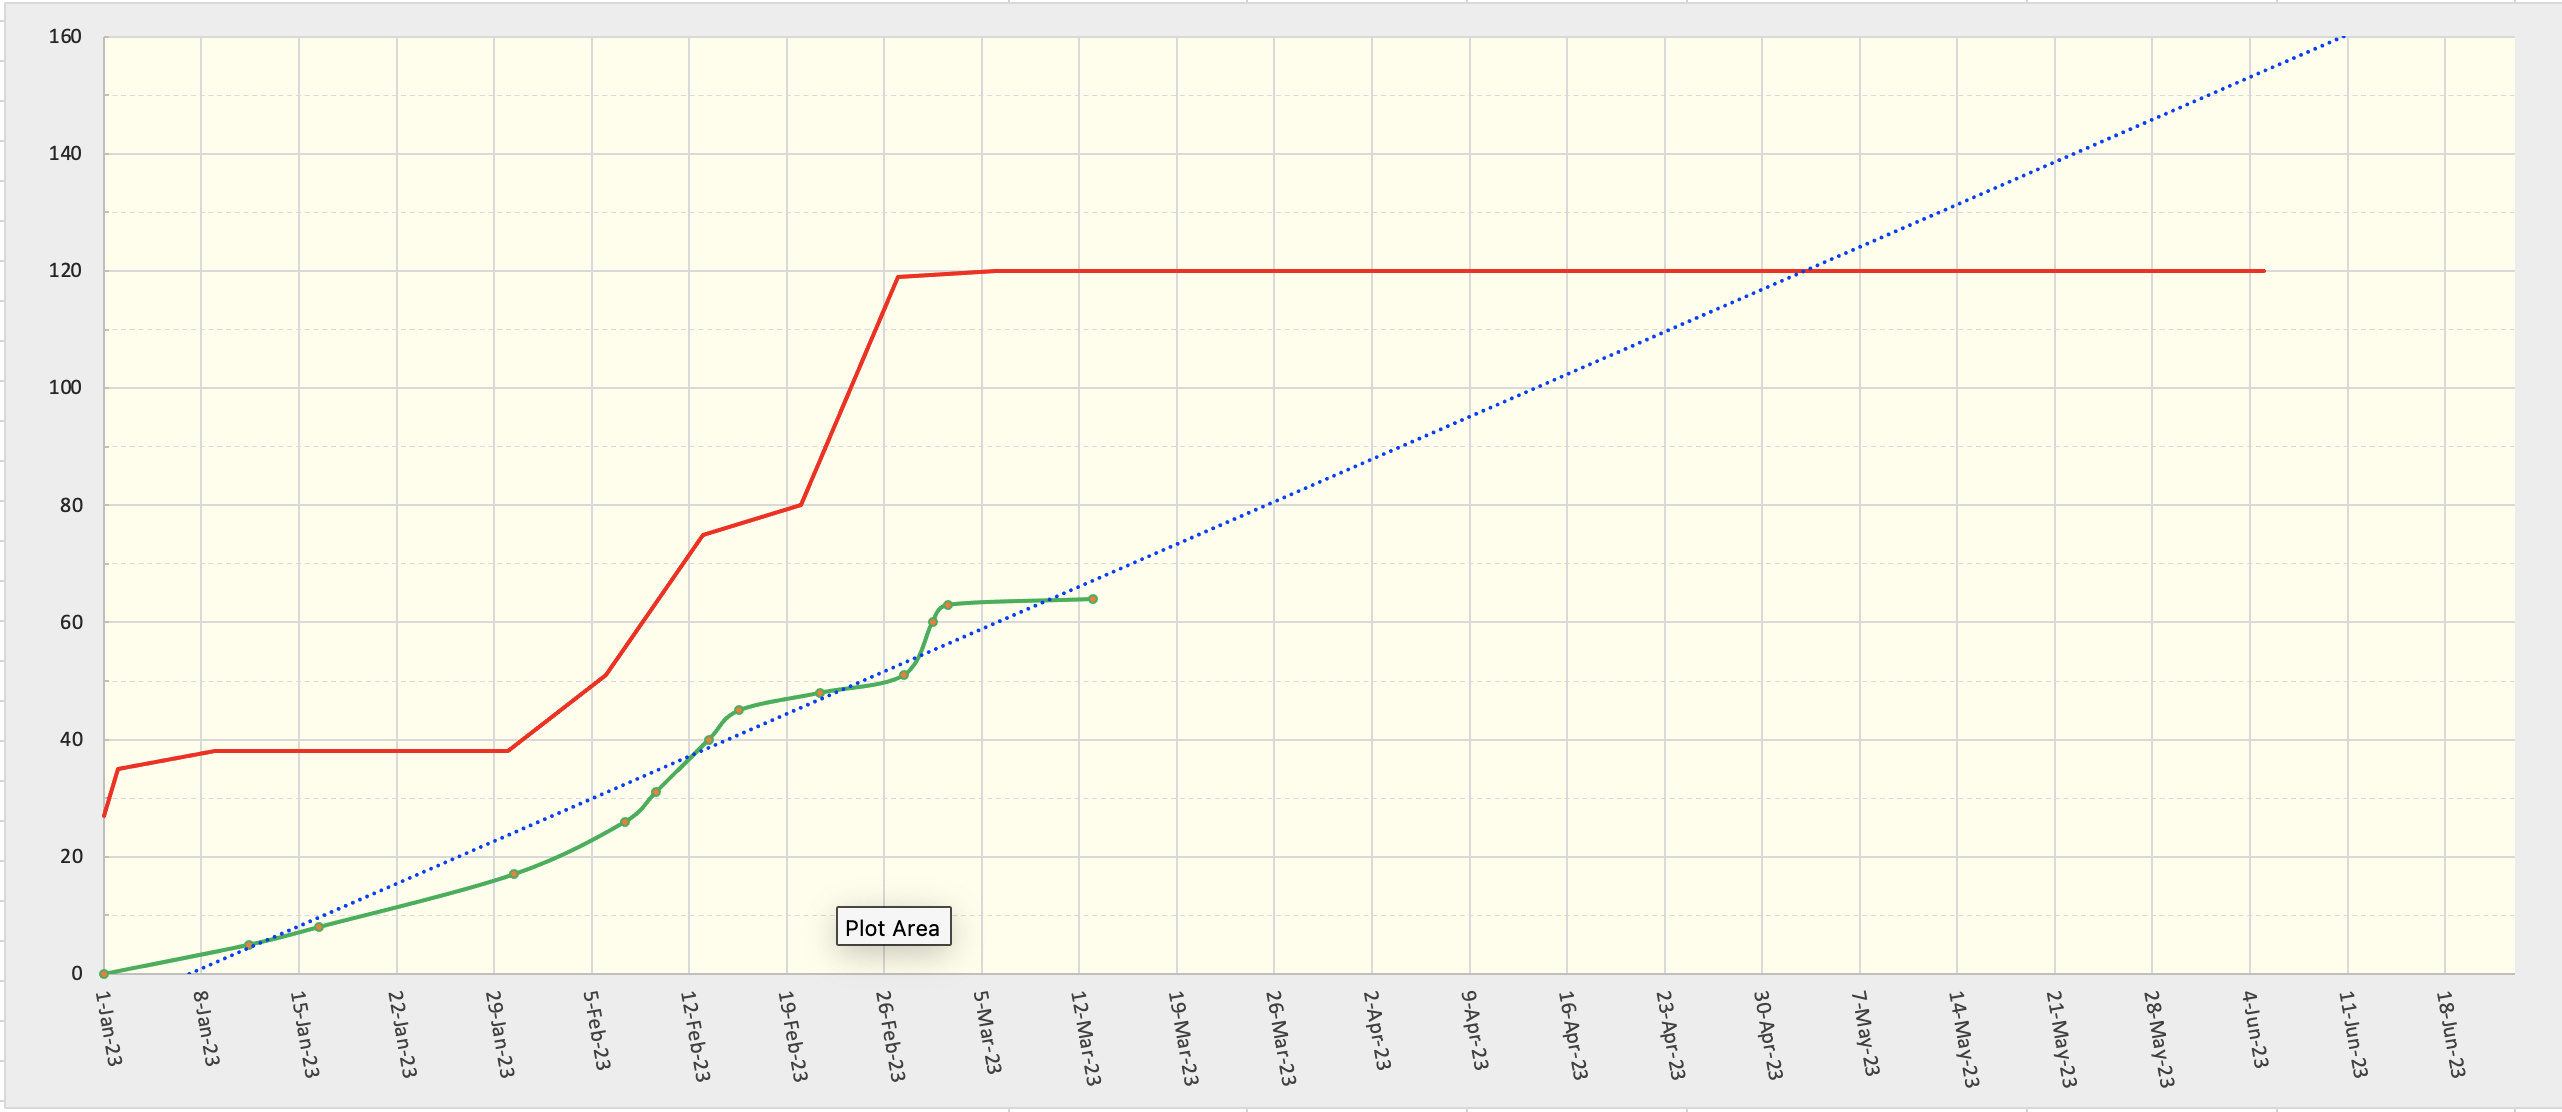
\includegraphics[width=6cm]{assets/burnup/2023-03-14.png}
    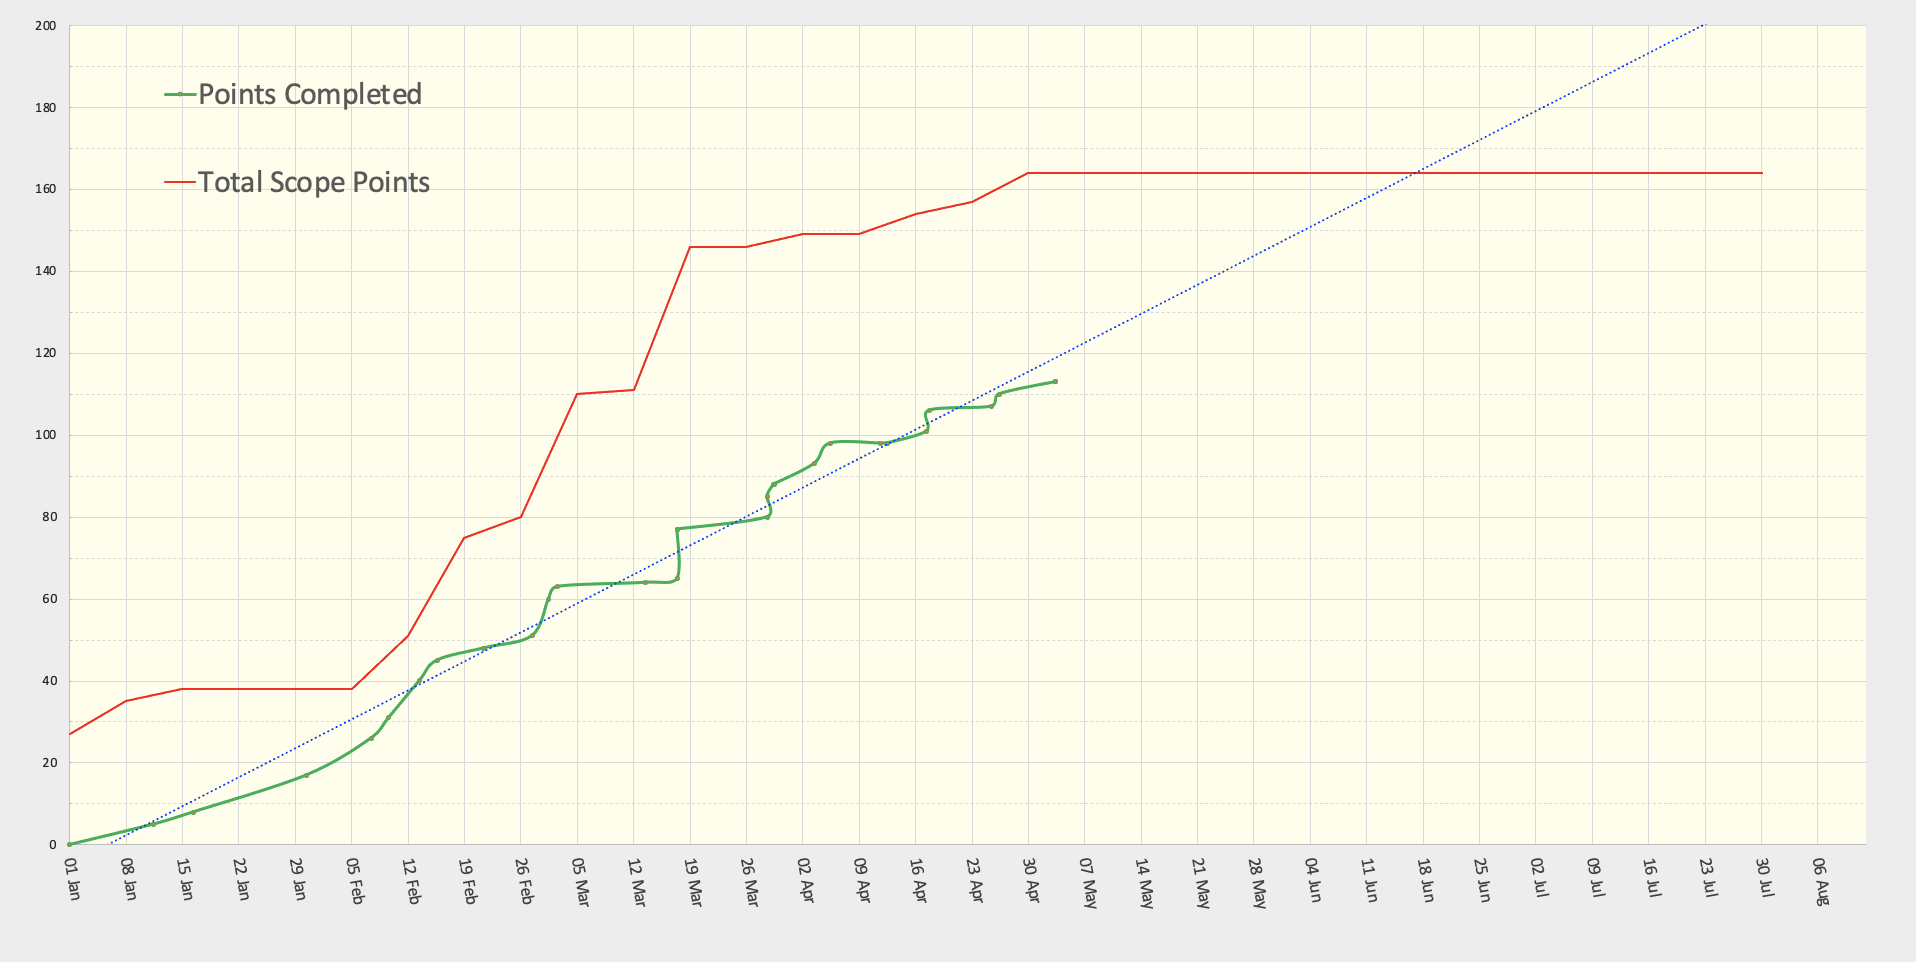
\includegraphics[width=6cm]{assets/burnup/2023-05-03.png}
    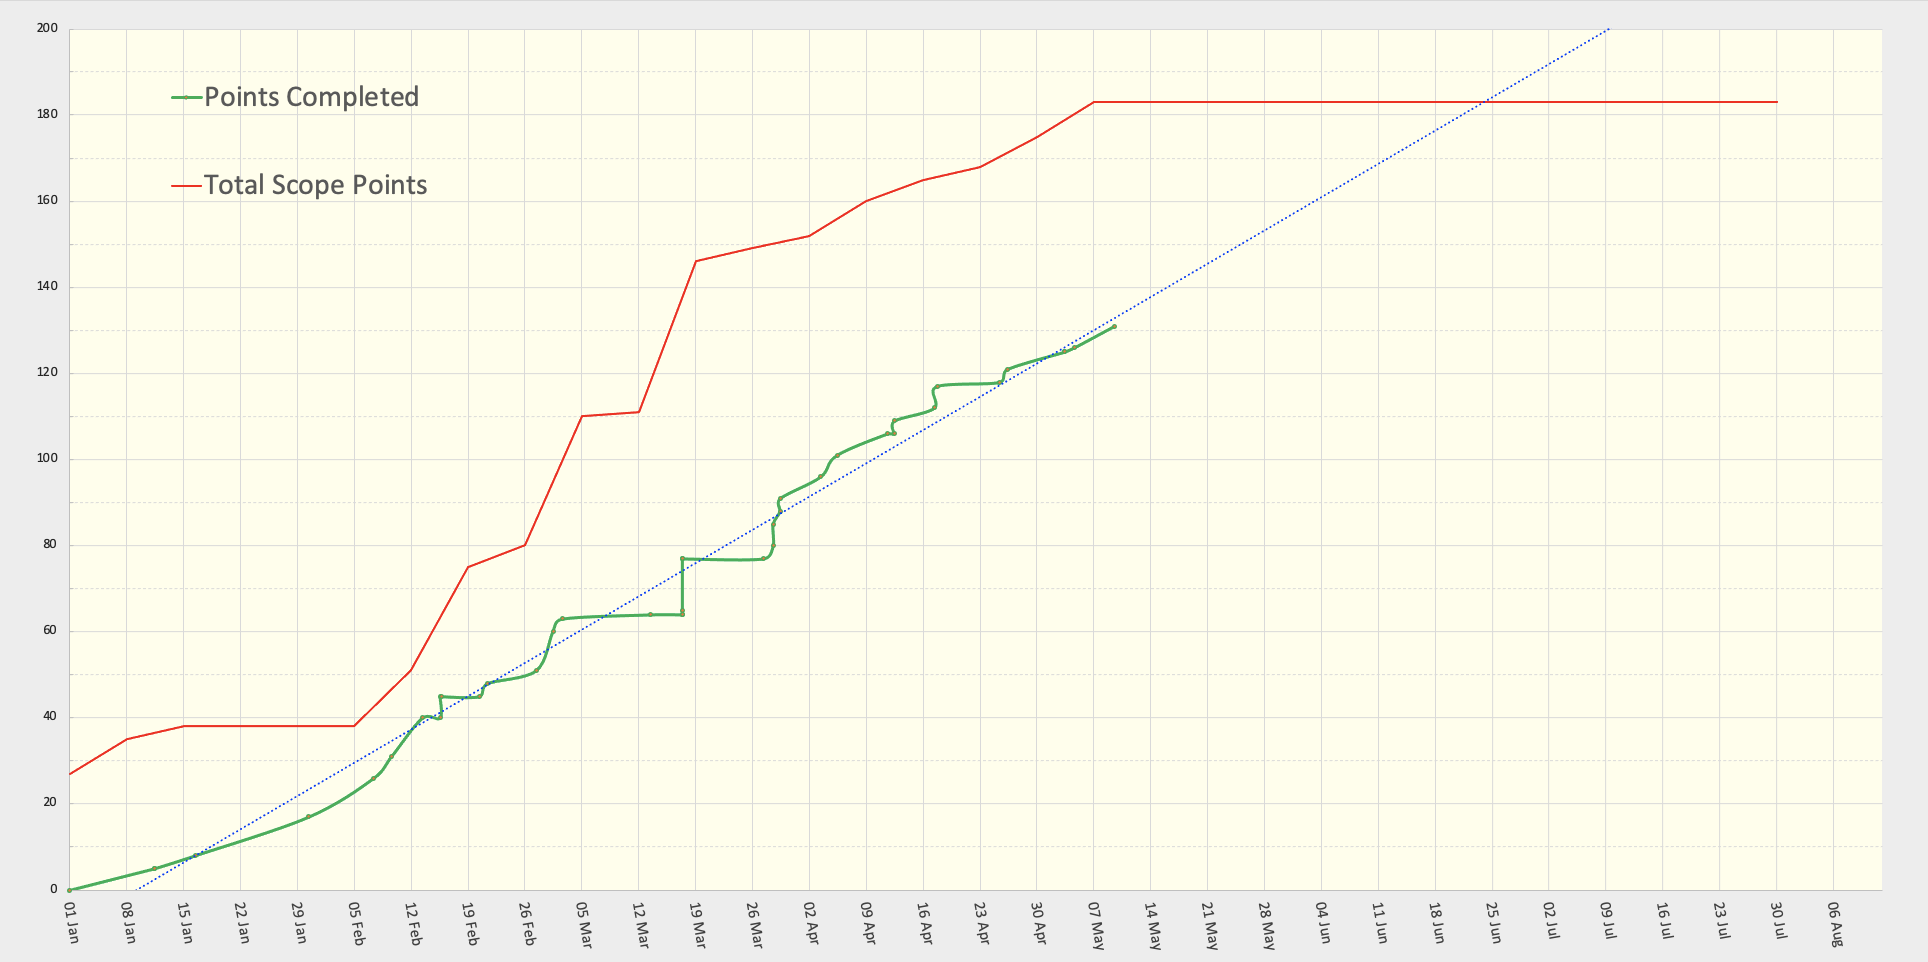
\includegraphics[width=6cm]{assets/burnup/2023-05-10.png}
    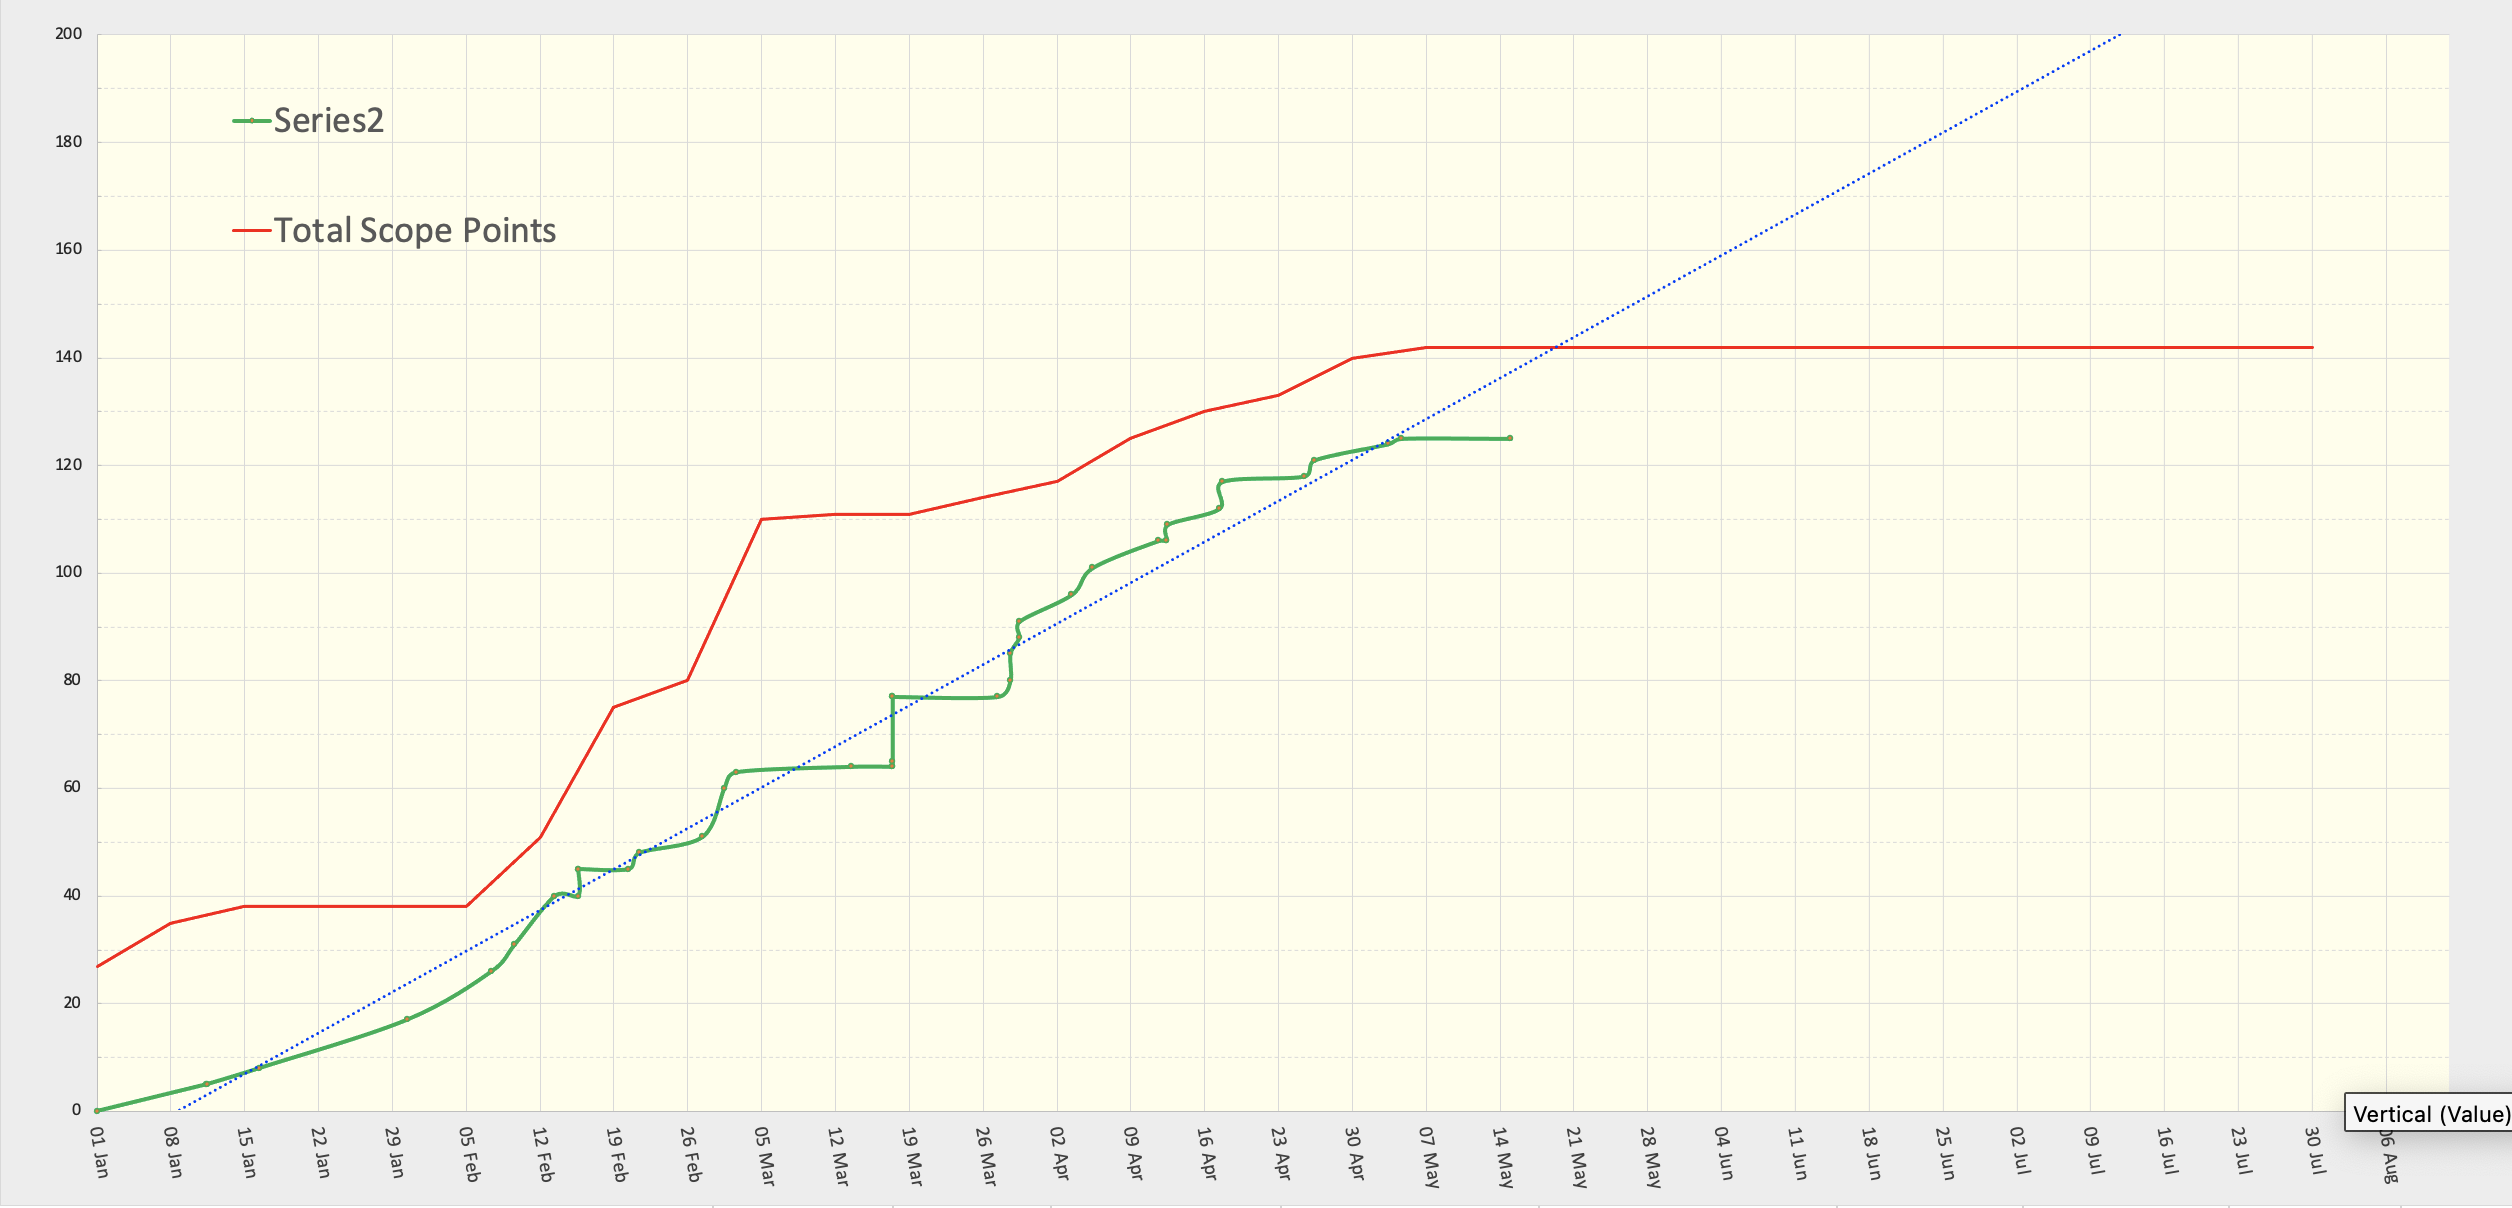
\includegraphics[width=6cm]{assets/burnup/2023-05-15.png}
    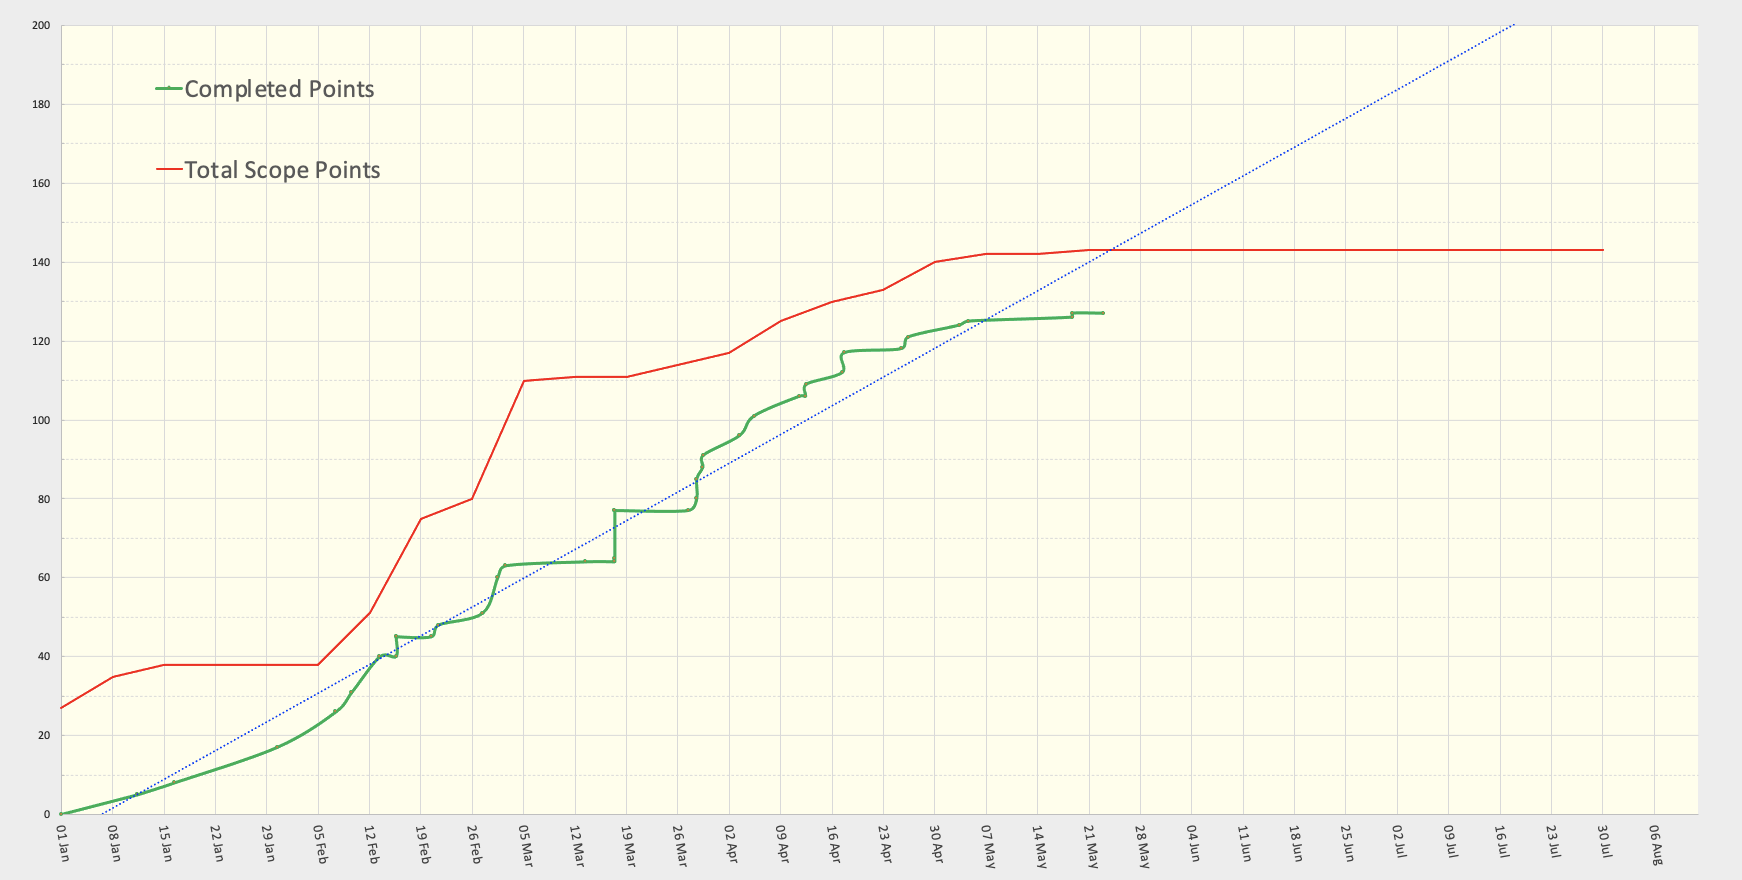
\includegraphics[width=6cm]{assets/burnup/2023-05-23.png}
    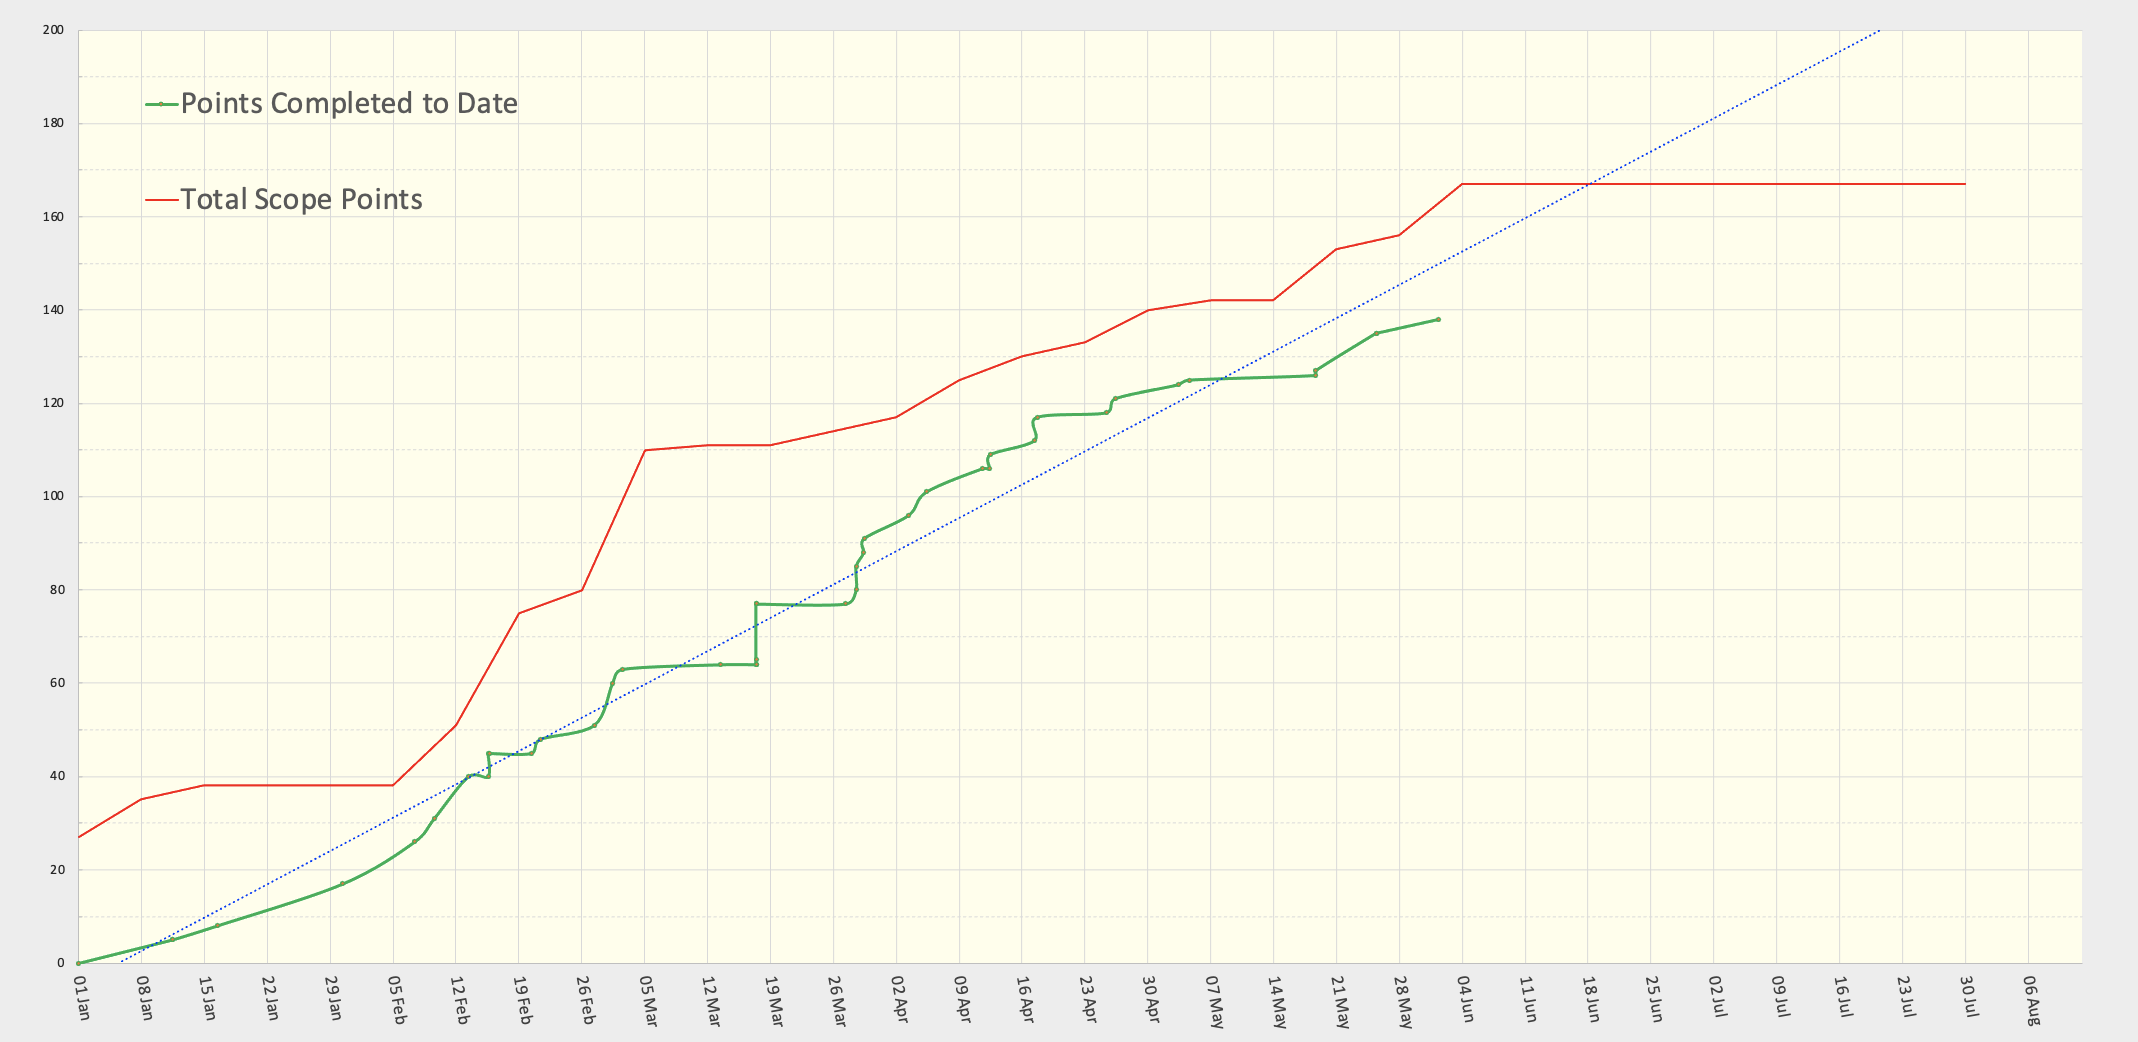
\includegraphics[width=6cm]{assets/burnup/2023-06-03.png}
    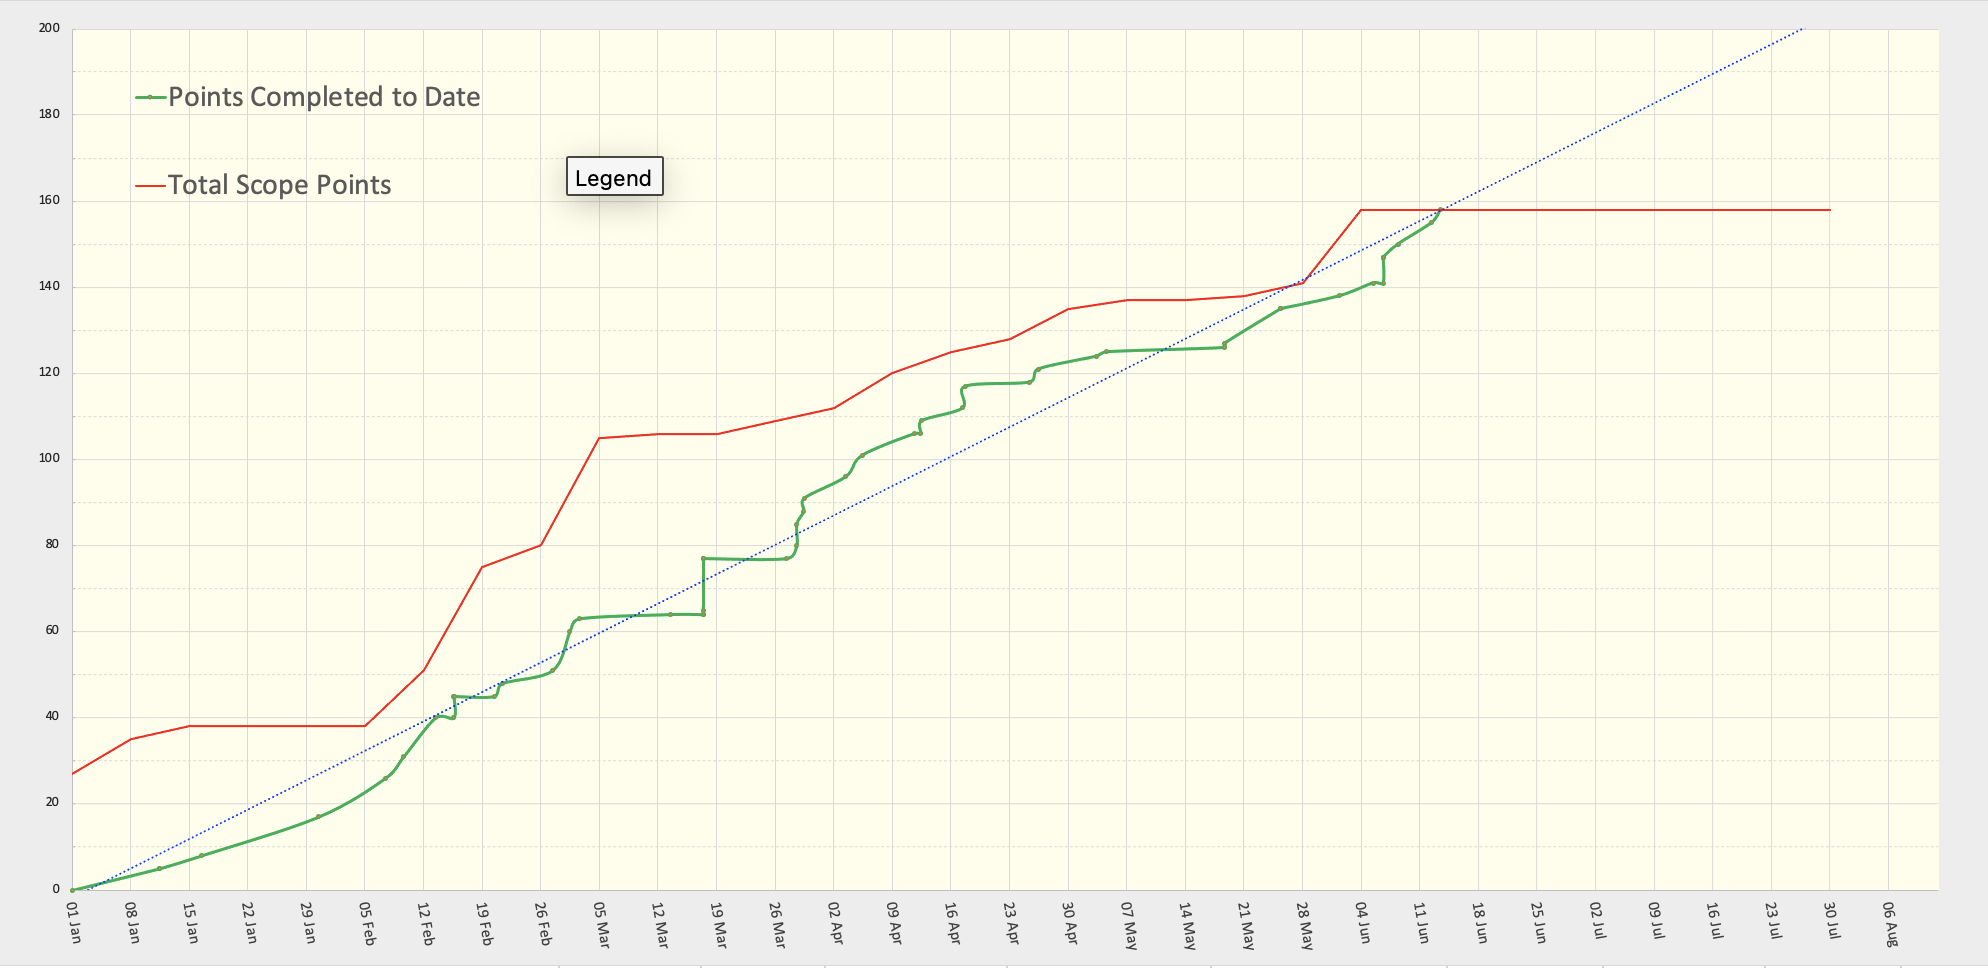
\includegraphics[width=6cm]{assets/burnup/2023-06-13.png}
    \caption{Exported graph of burn-ups overtime.}
    \label{fig:scheduleBurnup}
  \end{figure}

  The red line represents total amount of work todo, the dotted blue line is the expected projection of work completed overtime and the green line 
  is the amount of worked actually completed. As we discovered more work the we gradually got behind at first, however then began to get back 
  on track. Then scope creep, asks and deliverables [that] exceed the pre-set project scope [TODO2], kicked in as we added deltas to the MVP. As discussed 
  above this was then changed to come after and we were then able to finish on time.

  I found this helpful during the process as you could gauge where we were up to in the project. As well as the dropping of deltas on the MVP, automated 
  tests were picked up by devs, not just QA, which also helped us speed up development towards the end. I think these are great for time sensitive
  projects, however may add unneeded scrutiny and pressure on non time-sensitive projects.

  \newpage

  \section{Off Product Inspector Tooling}

  The Off Product Inspector (OPI) was made so that people in editorial and partner marketing and non technical team members, could view the data that
  should be available to partners at that moment. It allows users to search for pids (unique identifiers) and titles of brands, series and episodes
  and then view the data of these items. I worked on two main things to extend this project, upgrade to support our new v2 catalogues and add the 
  Deeplink Generator.

  \subsection{Support v2 Catalogues}
  The OPI originally was designed to support the v1.1 catalogue, however the catalogue had been extended to v2 which included different data and also 
  had 3 \textit{horizon catalogues}.
  \begin{itemize}
    \item \textbf{v2.0 catalogue} - Contains all data, both what is currently available and unavailable on iPlayer.
    \item \textbf{v2.0 0-day catalogue} - Contains data that is on iPlayer right now.
    \item \textbf{v2.0 8-day catalogue} - Contains data that is on iPlayer right now and also contains things that will be available within 8 days.
  \end{itemize}

  Partners are being encouraged to move over to the new v2 version of the catalogue so its good to be able to see what theses catalogue should offer.
  Me and a fellow junior software engineer began by working on the \textit{spike} for the project. A spike is a task thats aim is to gain knowledge
  \todo[noline, size=\small]{B5, P3}
  and information on ahead of doing the work. This can often times mean creating a small MVP to show that it is possible. I talk about this and other
  software lifecycle issues in the \textbf{Software Engineering-1.pdf} document. The spike we created was an MVP that allowed the switching between 
  catalogue, however the code was not refined, there was no tests written and zero documentation, this would all come later. We then showed what we 
  had come up with to the team and then began the process of breaking the work down into slices/tickets.

  \vspace{0.2cm}

  I had never done or heard of a \textit{spike} before doing this for the OPI. It's easy to get carried away and go beyond the scope of the spike.
  Towards the end of this spike I began writing some tests for certain things but learned that this was not part of what a spike was. When doing 
  another spike for the schedules ingester, I took this lesson and stayed within the scope. This was also the first time I had been given a task that
  was UI based. \todo[noline, size=\small]{L2, L3, L7}
  This is an area I have much more knowledge in from my own teachings and allowed me to help/teach my colleague I was spiking with learn
  about how things like React hooks work and the interplay between React and Next.js.
  Further along in the project I also suggested that we move to a newer way of writing css and components called \textit{styled components}. Some benefits of
  these are:
  \todo[noline, size=\small]{T2}
  \begin{itemize}
    \item Styles are not separate from the component itself, making it easier to debug.
    \item Styled components can take props to easily customise aspects of a components style.
    \item Default html tags are given a more meaningful name, making it easier to understand the role of a tag.
  \end{itemize}

  Below is an example of the difference between using styled components and styling using SaSS (Syntactically Awesome Style Sheets).

  \begin{figure}[H]
    \centering
    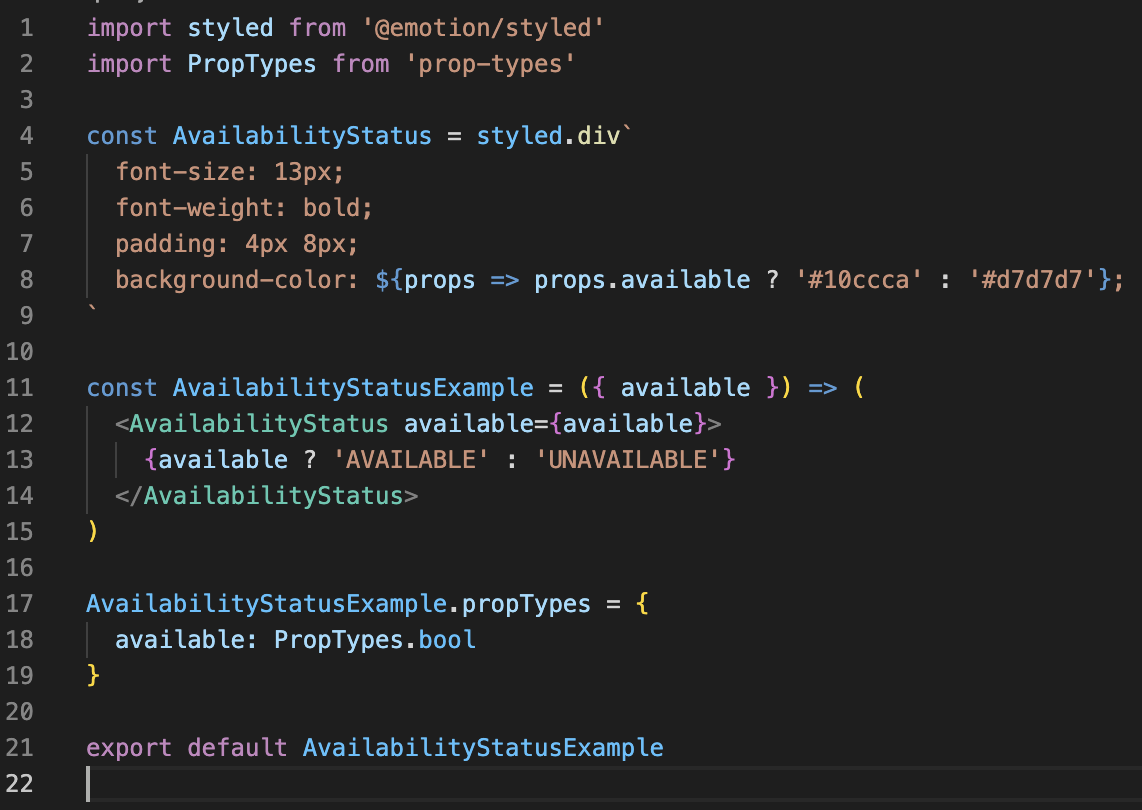
\includegraphics[width=6cm, height=4cm]{assets/StyledCompsOldJSX.png}
    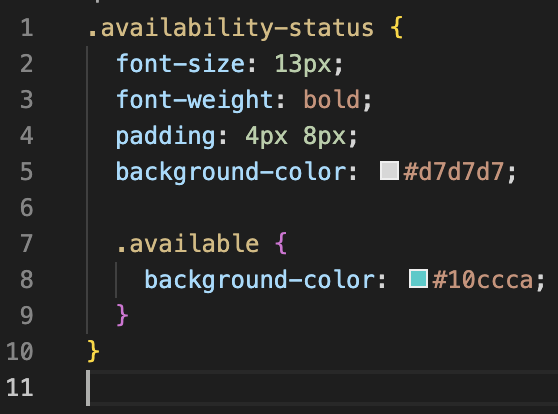
\includegraphics[width=6cm, height=4cm]{assets/styledCompsOldCSS.png}
    \caption{Screenshots of how not using styled components would work, JSX on left, SCSS on right.}
    \label{fig:oldStyling}
  \end{figure}

  \begin{figure}[H]
    \centering
    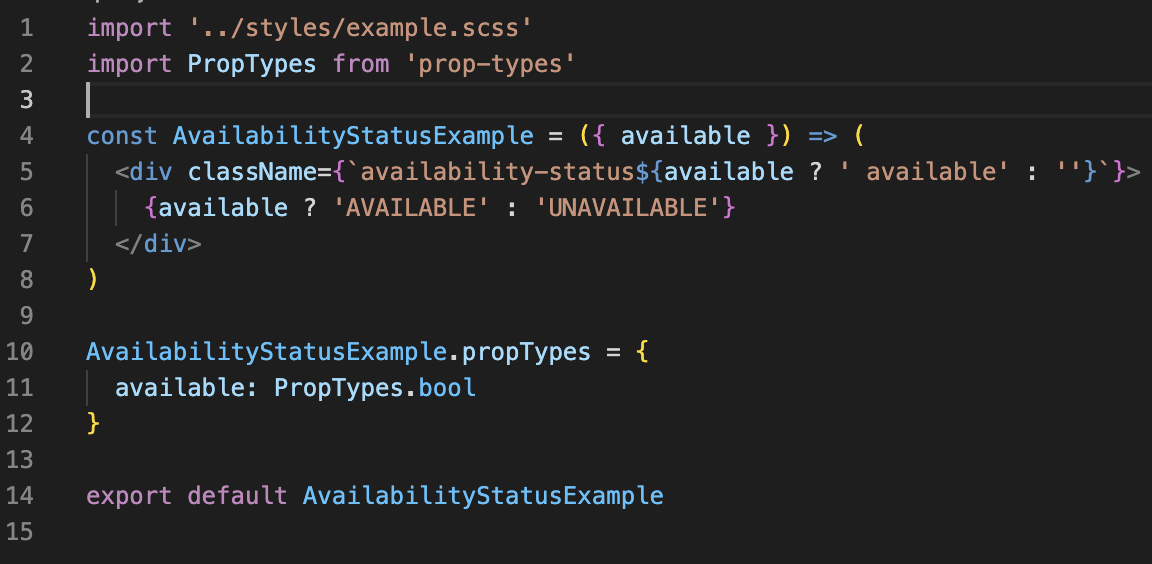
\includegraphics[width=8cm]{assets/styledCompsNew.png}
    \caption{Screenshot of how it looks using styled components.}
    \label{fig:newStyling}
  \end{figure}

  \subsection{Deeplink Generator}
  Deeplink generator stuff here.

    \subsubsection{Deeplink Generator Presentation}
    \todo[noline, size=\small]{P2, P3}
    On the 18th of July 2023 I presented at the Partnerships show n' tell meeting on behalf of my team. I presented the work we did for the
    deeplink generator and have included the slides in a separate document.

    This was the first time I've presented anything to a larger group of people and I was nervous going in. The presentation was short, due to the work
    being discussed not being very large, however it still took around 5 -7 minutes for the whole presentation. Overall I'm happy with how I managed the 
    presentation and with the presentation itself. It's something I should do more of in the future to become more comfortable with these kinds of things.
    For future I would take my time more when going through the slides. I felt like I rushed a little bit due to my nerves, however I feel like this is 
    something that comes with practice and being the the situation. 

  \subsection{Personal feedback on OPI}
  \todo[noline, size=\small]{P2, P3, L9, L10}
  I show the questions and feedback I received in the document \textbf{Feedback Form Output.docx}. I also go into a discussion of this in the document
  \textbf{Leaderships-1.pdf}.

  Reflecting now (August 2023) on the goals at the end of that assignment:
  \begin{itemize}
    \item \textbf{Pass AWS practitioner foundational} - I think I've outgrown this aim naturally. My skills and understanding of AWS is much greater than
    that of which I'd be assessed on. I am deffinately still interested in gaining some qualifications in AWS, however I would prefer for now to focus on 
    finishing my masters/apprenticeship rather than do that. In the future I will look into doing the develop or solutions architect certifications.
    \item \textbf{Improve input in meetings} - This is something I've got better at, partly due to me learning more about what we do as a team and therefore
    feeling less \textit{'imposter syndrome'} when giving out ideas.
    \item \textbf{Attend BBC mentoring training} - I am currently on the wait-list for this course.
  \end{itemize}

\newpage
  \subsection{B1 (Skill)}

  \begin{quote}
    \textit{'Identify, document, review, and design
    complex IT-enabled business processes that define a set
    of activities that will accomplish specific organisational
    goals and that provide a systematic approach to improving
    those processes.'}
  \end{quote}

\newpage
  \subsection{B2 (Skill)}

  \begin{quote}
    \textit{'Design and develop technology roadmaps,
    implementation strategies, and transformation plans
    focused on digital technologies in order to achieve
    improved productivity, functionality, and end-user
    experience in an area of technology specialization.'}
  \end{quote}

\newpage
  \subsection{B3 (Skill)}

  \begin{quote}
    \textit{'Deliver workplace transformations through
    planning and implementing technology-based business-
    change programmes, including setting objectives,
    priorities, and responsibilities with others in an area of
    technology specialization.'}
  \end{quote}

\newpage
  \subsection{B4 (Knowledge)}

  \begin{quote}
    \textit{'The strategic importance of technology
    enabled business processes, and how they are designed
    and managed in order to determine a firm’s ability to
    compete effectively.'}
  \end{quote}

\newpage
  \subsection{B5 (Knowledge)}

  \begin{quote}
    \textit{'The principles of business
    transformation and how organisations integrate different
    management functions in the context of technological
    change.'}
  \end{quote}

\newpage
  \subsection{B6 (Knowledge)}

  \begin{quote}
    \textit{'Own employer’s business objectives
    and strategy, its position in the market, and how it adds
    value to its clients through the services and/or products it
    provides.'}
  \end{quote}

\newpage
  \subsection{B7 (Knowledge)}

  \begin{quote}
    \textit{'How to justify the value of technology
    investments and apply benefits management and
    realisation.'}
  \end{quote}

\newpage

  \subsection{P1 (Skill)}

  \begin{quote}
    \textit{'Negotiate and agree digital-and-technology-
    specialism delivery budgets with those with decision-
    making responsibility.'}
  \end{quote}

\newpage
  \subsection{P2 (Skill)}

  \begin{quote}
    \textit{'Develop and deliver management level
    presentations which resonate with senior stakeholders,
    both business and technical.'}
  \end{quote}

\newpage
  \subsection{P3 (Skill)}

  \begin{quote}
    \textit{'Professionally present digital-and-technology-
    solution-specialism plans and solutions in a well-
    structured business report.'}
  \end{quote}

\newpage
  \subsection{P4 (Skill)}

  \begin{quote}
    \textit{'Demonstrate self-direction and originality in
    solving problems, and act autonomously in planning and
    implementing digital-and-technology-solution-specialist
    tasks at a professional level.'}
  \end{quote}

\newpage
  \subsection{P5 (Skill)}

  \begin{quote}
    \textit{'Be competent at negotiating and closing
    techniques in a range of interactions and engagements,
    both with senior internal stakeholders and external
    stakeholders.'}
  \end{quote}

\newpage
  \subsection{P6 (Knowledge)}

  \begin{quote}
    \textit{'The role of learning and talent
    management in successful business operations.'}
  \end{quote}

\newpage

  \subsection{L1 (Skill)}

  \begin{quote}
    \textit{'Evaluate the significance of human factors to
    leadership in the effective implementation and
    management of technology-enabled business processes.'}
  \end{quote}

\newpage
  \subsection{L2 (Skill)}

  \begin{quote}
    \textit{'Develop own leadership style and professional
    values that contribute to building high-performing teams.'}
  \end{quote}

\newpage
  \subsection{L3 (Behaviour)}

  \begin{quote}
    \textit{'Inspire and motivate others to deliver
    excellent technical solutions and outcomes.'}
  \end{quote}

\newpage
  \subsection{L4 (Behaviour)}

  \begin{quote}
    \textit{'Establish high levels of performance in
    digital and technology solutions activities.'}
  \end{quote}

\newpage
  \subsection{L5 (Behaviour)}

  \begin{quote}
    \textit{'Be results and outcomes driven in order
    to achieve high key performance outcomes for digital and
    technology solutions objectives.'}
  \end{quote}

\newpage
  \subsection{L6 (Behaviour)}

  \begin{quote}
    \textit{'Promote a high level of cooperation
    between own work group and other groups in order to
    establish a technology-change led culture.'}
  \end{quote}

\newpage
  \subsection{L7 (Behaviour)}

  \begin{quote}
    \textit{'Develop and support others in
    developing an appropriate balance of leadership and
    technical skills.'}
  \end{quote}

\newpage
  \subsection{L8 (Behaviour)}

  \begin{quote}
    \textit{'Create strong positive relationships with
    team members to produce high-performing technical
    teams.'}
  \end{quote}

\newpage
  \subsection{L9 (Knowledge)}

  \begin{quote}
    \textit{'The role of leadership in contemporary
    technology-based organisations.'}
  \end{quote}

\newpage
  \subsection{L10 (Knowledge)}

  \begin{quote}
    \textit{'The personal leadership qualities that
    are required to establish and maintain an organisation’s
    technical reputation.'}
  \end{quote}

\newpage
  \subsection{L11 (Knowledge)}

  \begin{quote}
    \textit{'The role of leaders as change agents,
    and the identity of contributors to successful
    implementation.'}
  \end{quote}

\newpage

  \subsection{T1 (Skill)}

  \begin{quote}
    \textit{'Apply broader technical knowledge, combined
    with an understanding of the business context and how it
    is changing, in order to deliver to the company’s business
    strategy.'}
  \end{quote}

\newpage
  \subsection{T2 (Skill)}

  \begin{quote}
    \textit{'Demonstrate effective technology-leadership
    and change-management skills for managing technology-
    driven change and continuous improvement.'}
  \end{quote}

\newpage
  \subsection{T3 (Skill)}

  \begin{quote}
    \textit{'Create and implement innovative technological
    strategies in order to support the development of new
    products, processes, and services that align with the
    company’s business strategy, and develop and
    communicate compelling business proposals to support
    the strategies.'}
  \end{quote}

\newpage
  \subsection{T4 (Knowledge)}

  \begin{quote}
    \textit{'How to monitor technology related
    market trends and research and collect competitive
    intelligence.'}
  \end{quote}

\newpage
  \subsection{T5 (Knowledge)}

  \begin{quote}
    \textit{'Technology road-mapping concepts and
    methods, and how to apply them.'}
  \end{quote}

\newpage

  \subsection{SE-S01 (Skill)}

  \begin{quote}
    \textit{'Architect, build, and support leading-edge
    concurrent-software platforms that are performant to
    industry standards and that deliver responsive solutions
    with good test coverage.'}
  \end{quote}

\newpage
  \subsection{SE-S02 (Skill)}

  \begin{quote}
    \textit{'Drive the technology-decision-making and
    development process for projects of varying scales,
    considering current technologies including DevOps and
    Cloud Computing, and evaluate different technology-
    design and implementation options, making reasoned
    proposals and recommendations.'}
  \end{quote}

\newpage
  \subsection{SE-S03 (Skill)}

  \begin{quote}
    \textit{'Develop and deliver distributed or semi-complex
    software solutions that are scalable, and that deliver
    innovative user experiences and journeys that encompass
    cross-functional teams, platforms, and technologies.'}
  \end{quote}

\newpage
  \subsection{SE-S04 (Skill)}

  \begin{quote}
    \textit{'Update current software products, improving
    their efficiency and functionality, and build new features
    to product specifications.'}
  \end{quote}

\newpage
  \subsection{SE-S05 (Skill)}

  \begin{quote}
    \textit{'Accomplish planned software-development tasks
    that deliver the expected features within specified time
    constraints, security, and quality requirements.'}
  \end{quote}

\newpage
  \subsection{SE-S06 (Skill)}

  \begin{quote}
    \textit{'Be accountable for the quality of deliverables
    from one or more software-development teams (source
    code quality, automated testing, design quality,
    documentation, etc.), and following company-standard
    processes (code reviews, unit testing, source code
    management, etc.).'}
  \end{quote}

\newpage

  \subsection{SE-K01 (Knowledge)}

  \begin{quote}
    \textit{'The rationale for software-platform and solution
    development, including the organisational context.'}
  \end{quote}

\newpage
  \subsection{SE-K02 (Knowledge)}

  \begin{quote}
    \textit{'The various inputs, statements of requirements,
    security considerations, and constraints that guide solution
    architecture and the development of logical and physical
    systems’ designs.'}
  \end{quote}

\newpage
  \subsection{SE-K03 (Knowledge)}

  \begin{quote}
    \textit{'The methodologies designed to help create
    approaches for organizing the software-engineering
    process, the activities that need to be undertaken at
    different stages in the life-cycle, and techniques for
    managing risks in delivering software solutions.'}
  \end{quote}

\newpage
  \subsection{SE-K04 (Knowledge)}

  \begin{quote}
    \textit{'The approaches used to modularise the internal
    structure of an application, and to describe the structure
    and behaviour of applications used in a business, with a
    focus on how they interact with each other and with
    business users.'}
  \end{quote}

\newpage
  \subsection{SE-K05 (Knowledge)}

  \begin{quote}
    \textit{'How to design, develop, and deploy software
    solutions that are secure and effective in delivering the
    requirements of stakeholders, and the factors that affect
    the design of a successful code.'}
  \end{quote}

\newpage
  \subsection{SE-K06 (Knowledge)}

  \begin{quote}
    \textit{'The range of metrics which might be used to
    evaluate a delivered software product.'}
  \end{quote}

\newpage

  
\begin{landscape}
  \section{Appendix}
    \subsection{Appendix A - Full diagram of schedule pipeline infrastructure.}
      \begin{figure}[H]
        \centering
        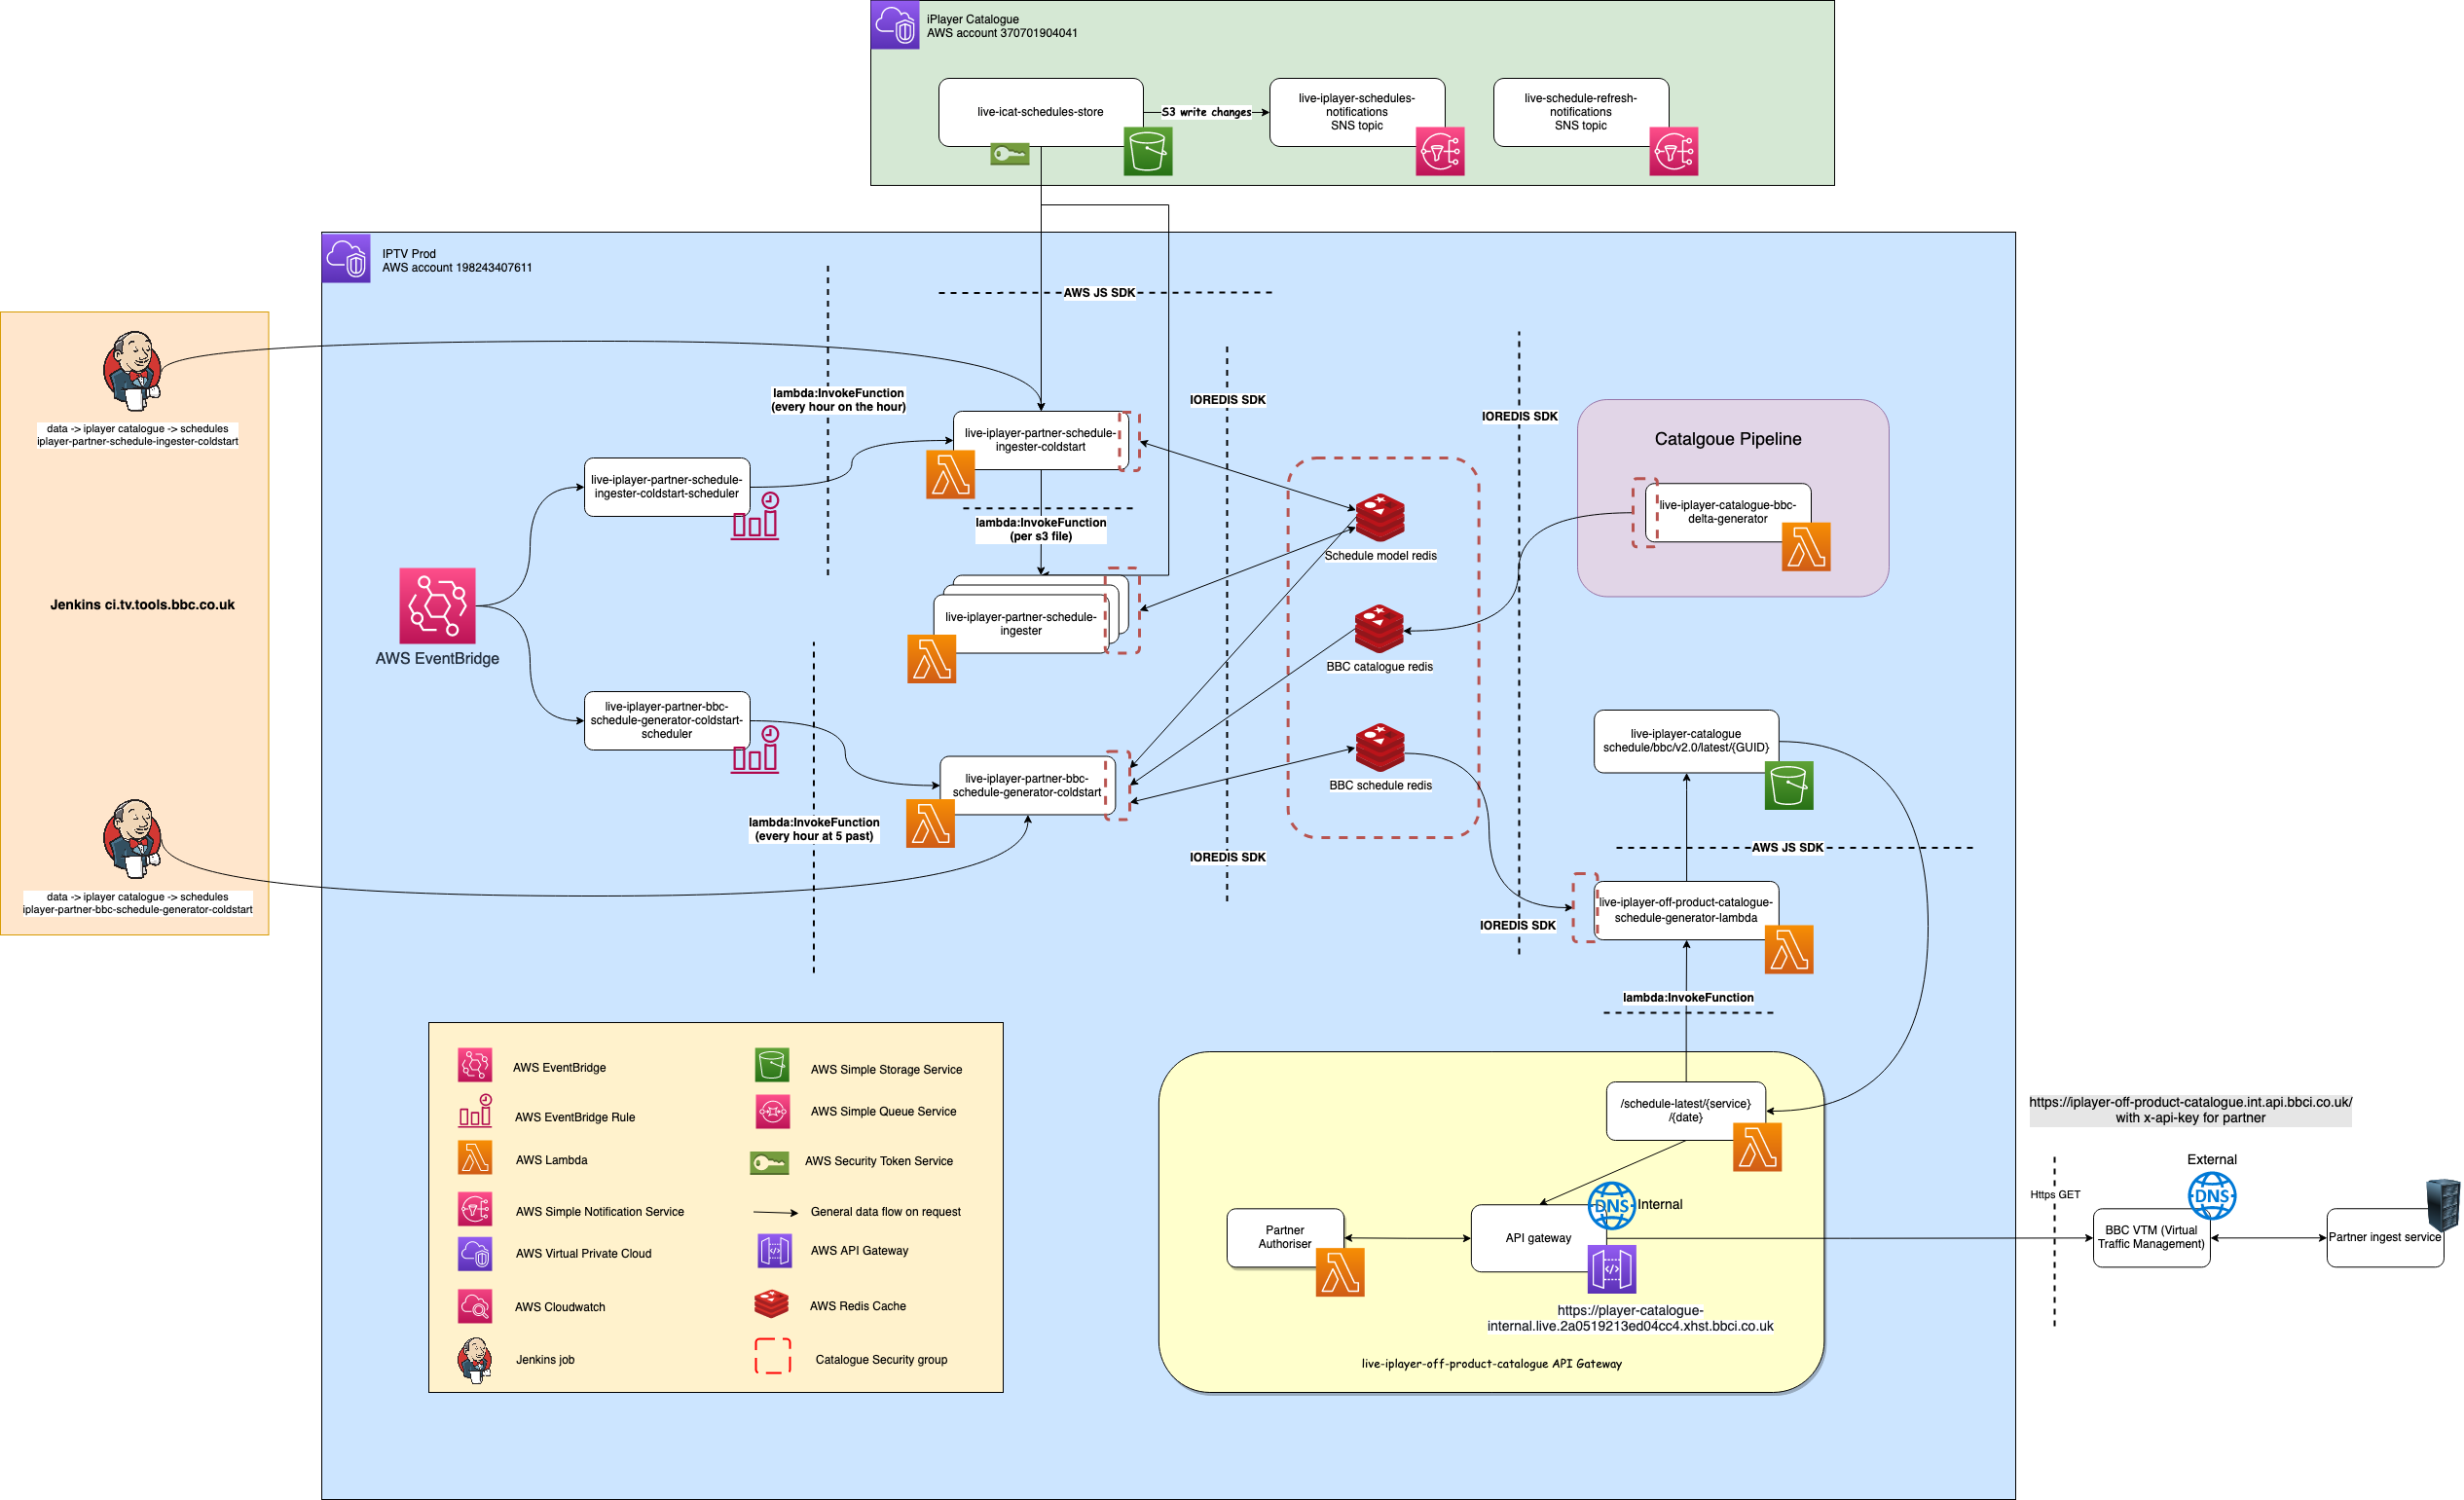
\includegraphics[width=18cm]{assets/schedulesThreatModel.drawio.png}
        \caption{Schedules threat model showing the entire pipeline.}
      \end{figure}  
\end{landscape}


\end{document}